% !TEX root = ../main.tex
\section{Projective \& Multiprojective Algebraic Geometry}
\subsection{Projective Algebraic Sets \& Projective Varieties}
\subsubsection{Basic Definitions}
    \begin{definition}
        Let $S\subset K[x_1,\dots,x_{n+1}]$ then we define \textit{the projective vanishing of $S$ over $K$} to be the set 
        $$V^{\Pp}(S) := V(S):= \{ [v]\in \Pp^n : [v] \text{ is a zero for every } f\in S\}$$
    \end{definition}
    \begin{definition}
        A set $X\subset \Pp^n$ is said to be a \textit{projective algebraic set} if 
        $$X =V(S)$$
        for some $S\subset K[x_1,\dots,x_{n+1}]$. $X$ is called a \textit{(projective) hypersurface} if $X=V(F)$ for some homogeneous $F\in K[\mathbf{x}]$. If $\deg \ F = 1$ we call it a \textit{(projective) hyperplane}.   
    \end{definition}
    \begin{remark}
        One notes that the hyperplanes $V(x_i)$ are the $i$'th hyperplanes at infinity.
    \end{remark}
    \begin{proposition}
        Let $K$ be an infinite field, $S\subset K[x_1,\dots,x_{n+1}]$ and $I:=\langle S\rangle =\langle f_1,\dots,f_m\rangle \subset K[x_1,\dots,x_{n+1}]$. Write 
        $$f_i=\sum_{0}^{d_i} f_{ij},$$
        where $f_{ij}$ are forms of degree $j$. Then $$V(S)=V(I)= V(\{f_{ij} : 1\leq i\leq m, 0\leq j\leq d_i\}).$$
    \end{proposition}
    \begin{proof}
        The first equality is trivial and the second equality follows from Lemma~\ref{FormsInFormDecompVanish}.
    \end{proof}
    \begin{remark}\label{WeMayAssumeProjectiveAlgebraicSetsToBeVanishingSetsOverHomogeneousIdeals}
        It thus follows that if $X\subset \Pp^n$ is a projective algebraic set, we may assume that $X=V(F_1,\dots,F_m)$ for homogeneous polynomials $F_1,\dots,F_m\in K[x_1,\dots,x_{n+1}]$. As a consequence if given a homogeneous ideal $I\subset K[\mathbf{x}]$, then $V^\A(I)\setminus 0\neq \emptyset$ implies $V^\Pp(I)\neq \emptyset$. Indeed, we may write $I=\langle F_1,\dots,F_m\rangle$ for suitable homogeneous polynomials $F_1,\dots,F_m\in K[\mathbf{x}]$. Meaning if $v\in \A^{n+1}\setminus 0$ is a zero of each $F_i$, then so is $[v]$.      
    \end{remark}
    \begin{lemma}
        If $K[x_1,\dots,x_{n+1}]\supset M\supset M'$, then $V^\Pp(M)\subset V^\Pp(M')$.
    \end{lemma}
    \begin{proof}
        The proof is almost identical to the proof of Lemma~\ref{SetSupersetImpliesVanishingSetOfSetSubsets}.    
    \end{proof}
    \begin{lemma}\label{ProjectiveAlgebraicSubsetsAreClosedUnderIntersectionAndFiniteUnion}
    We collect the following results which are projective analogues of Lemma~\ref{AlgebraicSubsetsAreClosedUnderIntersectionAndFiniteUnion}
    \begin{enumerate}[(i)]
        \item Let $A$ be some indexing set. Consider a family of algebraic sets $\{X_\alpha\}_{\alpha\in A}$ in $\A^n$. Then $\bigcap_{\alpha} X_\alpha$ is an algebraic set.
        \item Consider algebraic sets $X,Y\subset \A^n$. Then $X\cup Y$ is algebraic. It follows by induction that $\bigcup_1^k X_i$ is algebraic for any finite sequence of algebraic sets $X_1,\dots,X_k$ in $\A^n$.  
    \end{enumerate}
\end{lemma}
\begin{proof}
    1. Writing $X_\alpha = V(I_\alpha)$ for homogeneous $I_\alpha$, we prove the statement in the same manner as for the affine case, i.e. by proving $\bigcap_\alpha X_\alpha =  V\left(\bigcup_\alpha I_\alpha\right)= V\left(\left\langle \bigcup_\alpha I_\alpha\right\rangle\right) = V\left(\sum_\alpha I_\alpha \right)$. The proof of this is identical to the one given in Lemma~\ref{AlgebraicSubsetsAreClosedUnderIntersectionAndFiniteUnion} 1.\\
    2. For homogeneous ideals $I,J\subset K[\mathbf{x}]$. We prove that $V(I)\cup V(J)=V(IJ)$ for which the proof is identical to that of Lemma~\ref{AlgebraicSubsetsAreClosedUnderIntersectionAndFiniteUnion} 2.
\end{proof}
\begin{example}
    \begin{enumerate}
        \item $V^\Pp(0)= \Pp^n$. Indeed $0([v])=0$ for every $[v]\in\Pp^n$.
        \item $V^\Pp(1)= \emptyset$. Indeed $1(v)=1\neq 0$ for every $v\in \A^{n+1}\setminus 0$.
        \item $V^\Pp(x_1-x_{n+1}a_1,\dots,x_n-x_{n+1}a_n) = \{[(a_1,\dots,a_n,1)]\}$. Indeed, set $v=a_1,\dots,a_n,1)\in \A^{n+1}$. Then evaluating each of the $n$ polynomials in $\lambda v$ for $\lambda\in K\setminus 0$, we get $0$. Conversely if $w_i=w_{n+1}a_i$ for each $i$, note that necessarily $w_{n+1}\neq 0$, hence $(w_1,\dots,w_{n+1})=w_{n+1}v$, hence $[w]=[v]$. After permutation of indices we see that any point in $\Pp^n$ is a projective algebraic set, hence any finite subset of $\Pp^n$ is algebraic
    \end{enumerate}
\end{example}
\begin{remark}
    The system 
    $$\tau_\mathcal{Z} := \left\{ \Pp^n\setminus X : X\subset \Pp^n \text{ is an algebraic set} \right\}$$
    (analogously to the affine case) defines a topology on $\Pp^n$ which we also call \textit{Zariski topology}.
\end{remark}
    \begin{definition}
        For a set $X\subset \Pp^n$ we form 
        $$I^{\Pp}(X):=I(X):=\{ f\in K[x_1,\dots,x_n]: f([v]) \text{ for every } [v]\in X\}$$
        which we call the \textit{(homogeneous) ideal of $X$}
    \end{definition}
    \begin{remark}
        The above set is a homogeneous ideal. That it is an ideal is trivial. Again by Lemma~\ref{FormsInFormDecompVanish} it is homogeneous. We also have that $I(X)$ is generated by a finite set of homogeneous polynomials due to Lemma~\ref{HomogeneousIdealsAreGeneratedByForms}. 
    \end{remark}
    \begin{lemma}
        If $X,Y\subset \Pp^n$ are algebraic such that $X\subset Y$, then $I(X)\supset I(Y)$.
    \end{lemma}
    \begin{proof}
        The proof is identical to the affine case
    \end{proof}
    \begin{lemma}\label{ProjectiveIdealVanishingSets}
    Let $M \subset K[x_1,\dots,x_{n+1}]$ and $X\subset \Pp^n$. Then we have the following
    \begin{enumerate}
        \item $I(V(M)) \supset M$.
        \item $V(I(X)) \supset X$.
        \item $V(I(V(M)))=V(M)$. Hence if $X$ is algebraic $X=V(I(X))$.
        \item $I(V(I(X)))=I(X)$. Hence if $M$ is an ideal of some algebraic set, $M= I(V(M))$
    \end{enumerate}
    \end{lemma}
    \begin{proof}
        The proof is identical to the affine case.    
    \end{proof}
    \begin{lemma}
        Let $X\subset \A^n$. Then $I(X)$ is radical. 
    \end{lemma}
    \begin{proof}
        The proof is identical to the affine case.
    \end{proof}
    \begin{lemma}\label{ProjectiveI(.)IsInjective}
        Let $X,Y\subset \A^n$ be algebraic subsets. Then 
        $$X=Y \iff I(X) = I(Y).$$ 
    \end{lemma}
    \begin{proof}
        The proof is identical to the affine case.
    \end{proof}
    \begin{example}
        \begin{enumerate}
            \item $I(\emptyset)=K[x_1,\dots,x_{n+1}]$
            \item If $\#K=\infty$, $I(\Pp^n)=0$. Indeed, if $f([v])=0$ for every $[v]$, then $f_0([v])=0$, hence $f(0)=0$. It thus follows that $f(v)=0$ for every $v\in \A^{n+1}$, hence $f=0$.
            \item $I(\{[v_1,\dots,v_n,1]\})=\langle x_1-x_{n+1}v_1,\dots,x_n-x_{n+1}v_n\rangle$.
        \end{enumerate}
    \end{example}
    \begin{definition}
        An algebraic set is \textit{reducible} if can be written as the union of two strictly smaller algebraic set. It is called \textit{irreducible} or \textit{a (projective) variety}, if it is not reducible.
    \end{definition}
    \begin{lemma}
        An algebraic set $V\subset \Pp^n$ is a variety if and only if $I(V)$ is prime if and only if $K[x_1,\dots,x_{n+1}]/I(V)$ is an integral domain.
    \end{lemma}
    \begin{proof}
        "$\implies$": Suppose $I(V)$ is not prime. Then there are homogeneous $F_1,F_2\in K[x_1,\dots,x_{n+1}]\setminus I(V)$ such that $F_1F_2\in I(V)$, by Lemma~\ref{CheckingHomogeneousIdealPrimeSufficesToCheckForms}. Then $V\cap V(F_i)\subsetneq V$ and 
        $$V= V\cap V(F_1F_2)=(V\cap V(F_1))\cup(V\cap V(F_2)).$$
        "$\impliedby$": Conversely if $V=V_1\cup V_2$ where $V_i\subsetneq V$, then $I(V_i)\supsetneq I(V)$. Pick $F_i\in I(V_i)\setminus I(V)$, then $F_1F_2\in I(V_1\cup V_2)=I(V)$, hence $I(V)$ is not prime.  
    \end{proof}
    Again using that $K[x_1,\dots,x_{n+1}]$ is noetherian, we can prove that any projective algebraic set has unique decomposition into a union of projective varieties.
\subsubsection{The Cone of a Projective Algebraic Set}
    \begin{definition}
        Let $X\subset \Pp^n$ be algebraic. We define \textit{the cone over $X$} to be the set 
        $$C(X):=\{v\in \A^{n+1}: [v]\in X \text{ or } v=0\}.$$
    \end{definition}
    \begin{lemma}\label{ProjectiveAndAffineIdealsOfNonEmptyProjectiveSetsRespectivelyItsConeAgree}
        Let $V\subset \Pp^n$ be a non-empty algebraic set. Then 
        $$I^\A(C(V))=I^\Pp(V).$$
    \end{lemma}
    \begin{proof}
        "$\subset$": Let $f\in I^\A(C(V))$ and $[v]\in V$. Then $\lambda v\in C(V)$ for every $\lambda\in K\setminus 0$, meaning $f(\lambda v)=0$. Then $f([v])=0$, hence $f\in I^\Pp(V)$.\\
        "$\supset$": Let $f\in I^\Pp(V)$ and $v\in C(V)$. If $[v]\in V$, then $f([v])=0$, hence in particular $f(v)=0$. If $v=0$, note that writing $f=\sum_0^d f_i$, we get that $f_i(w)=0$ for a $[w]\in V$, hence $f_i = 0$. Then trivially $f(0)=0$.
    \end{proof}
    \begin{lemma}\label{EqualityOfConeAndAffineVanishingSet}
        If $I\subset K[x_1,\dots,x_{n+1}]$ is homogeneous, then $V^\Pp(I)\neq  \emptyset$ implies $C(V^\Pp(I))=V^\A(I)$
    \end{lemma}
    \begin{proof}
         "$\subset$": Let $v\in C(V^\Pp(I))$ and $f=\sum_0^d f_i\in I$. Then if $[v]\in V^\Pp(I)$, $f([v])=0$, hence $f(v)=0$. If $v=0$, then for a given $[w]\in V^\Pp(I)$, $f_i([w])=0$, hence $f_i=0$, meaning $f_i(0)=0$. In any case $v\in V^\A(I)$.\\
        "$\supset$": Let $v\in V^\A(I)$ and $f=\sum_0^d f_i\in I$. If $v=0$, then $v\in C(V^\Pp(I))$ trivially. So suppose $v\neq 0$. Note that $f_i(v)=0$ for each $i$ since $f_i\in I$, hence $f_i(\lambda v)=0$ for each $\lambda\in K\setminus 0$. It thus follows that $f([v])=0$, hence $v\in C(V^\Pp(I))$.
    \end{proof}
    \begin{lemma}
        If $I\subset K[x_1,\dots,x_{n+1}]$ is homogeneous and not contained in $\langle x_1,\dots,x_{n+1}\rangle$, then $V^\Pp(I)\neq \emptyset$ if and only if $C(V^\Pp(I))=V^\A(I)$. In the case $I\not\subset \langle x_1,\dots,x_{n+1}\rangle$, $V^\A(I)= \emptyset$. In the case $I=\langle x_1,\dots,x_{n+1}\rangle^d$, then $C(V^\Pp(I))=\{0\}=V^\A(I)$.
    \end{lemma}
    \begin{proof}
        "$\implies$": Follows immediately from the prior lemma.\\
        "$\impliedby$": If $V^\Pp(I)= \emptyset$, then $C(V^\Pp(I))=\{0\}$ and $V^\A(I)\setminus 0 = \emptyset$ (cf. Remark~\ref{WeMayAssumeProjectiveAlgebraicSetsToBeVanishingSetsOverHomogeneousIdeals}). Note also that "$\supset$" in the prior lemma holds true in any case. Then $V^\A(I)\in\{\emptyset, \{0\}\}$. If $V^\A(I)=\{0\}$, then $I\subset I(V^\A(I))=\langle x_1,\dots,x_n\rangle$, so we conclude that $V^\A(I)=\emptyset\subsetneq \{0\}= C(V^\Pp(I))$.\\
        If $I=\langle x_1,\dots,x_{n+1}\rangle^d$, then $v\in V^\A(I) \iff v=0$, hence $V^\Pp(I)=\emptyset$
    \end{proof}
    \begin{proposition}
        Each irreducible component of a cone $C(V^\Pp(I))$ is itself a cone.  
    \end{proposition}
    \begin{proof}
        \textbf{Claim:} Let $W\subset V^\Pp(I)$ be a component of $V^\Pp(I)$. Then $C(W)\subset C(V^\Pp(I))$ is a component. Suppose $V:= V^\Pp(I) = V_1\cup V_2$ with $V_i\subsetneq V$. Then there is a $[v_i]\in V$ such that $[v_i]\notin V_i$. Then $v_i\in C(V)\setminus C(V_i)$.\\
        Let $U$ be a component of $C(V)$. By uniqueness of decomposition into components $U=C(W)$ for some component of $V$.
    \end{proof}
\subsubsection{The Projective Nullstellensatz}
    \begin{lemma}\label{PNSLemma}
        Let $I\subset K[x_1,\dots,x_{n+1}]$ be an homogeneous ideal. The following are equivalent.
        \begin{enumerate}
            \item $V^\Pp(I)=\emptyset$.
            \item $V^\A(I)\subset \{0\}$.
            \item $\rad(I)=I^\A(V^\A(I))\supset \langle x_1,\dots,x_{n+1}\rangle$.
            \item $\langle x_1,\dots,x_{n+1}\rangle^d \subset I $ for a suitably large $d\geq 0$
        \end{enumerate}
    \end{lemma}
    \begin{proof}
        "1. $\iff$ 2.": This follows from the prior lemma. "2. $\iff$ 3.": This follows from HNS. "3. $\iff$ 4.": This follows from Lemma~\ref{RadicalLemma}.
    \end{proof}
    \begin{theorem}\label{ProjectiveNullstellenSatz}(Projective Nullstellensatz/PNS)\\
        Let $I\subset K[x_1,\dots,x_{n+1}]$ be a homogeneous ideal. Then 
        \begin{enumerate}
            \item $V^\Pp(I)=\emptyset $ if and only if $V(d,n+1)\subset I$ for some $d\geq 0$.
            \item If $V^\Pp(I)\neq \emptyset$, then $I^\Pp(V^\Pp(I))=\rad(I)$.
        \end{enumerate}
    \end{theorem}
    \begin{proof}
        1. Is an immediate consequence of the above lemma.\\
        2. By Lemma~\ref{EqualityOfConeAndAffineVanishingSet} $V^\A(I)=C(V^\Pp(I))$ and by Lemma~\ref{ProjectiveAndAffineIdealsOfNonEmptyProjectiveSetsRespectivelyItsConeAgree}
        $$I^\Pp(V^\Pp(I))=I^\A(C(V^\Pp(I)))=I^\A(V^\A(I))=\rad(I),$$
        where the last equality is just HNS.
    \end{proof}
    {\Large write relevant corollaries to the PNS}
    \subsubsection{Rational Functions and Local Rings of Projective Varieties}
    \begin{definition}
        For a projective variety, $V\subset \Pp^n$ we define the \textit{homogeneous coordinate ring of $V$} to be the integral domain (recall that $I(V)$ is prime)
        $$\Gamma^h(V):= \Gamma(V):= K[\mathbf{x}]/I^\Pp(V).$$
    \end{definition}
    \begin{remark}
        In general it is not true that the homogeneous coordinate ring can be thought of as a subring of $\Fun(V,K)$, indeed consider for example $f=\sum_0^d f_i\in K[x_1,\dots,x_n]$, then for a $v\in \A^{n+1}\setminus 0$, $f(\lambda v) = \sum_0^d \lambda^if_i(v)$. Note then that the function $\lambda \mapsto f(\lambda v)$ is constant if and only if $f_i=0$ for $i>0$. Hence for some $\lambda,\lambda'\in K\setminus 0$, $f(\lambda v)\neq f(\lambda'v)$, meaning $f([v])$ is not well-defined unless $f$ is constant. What then can be said is that for $V\neq \emptyset$, $\{c + I(V) : c\in K\} \simeq \{ ([v]\mapsto c)\in \Fun(V,K): c \in K\}$, which is trivial. 
    \end{remark}
    \begin{definition}
        For a projective variety, $V\subset \Pp^n$ we define the \textit{homogeneous function field of $V$} to be the field 
        $$K^h(V):= Q(\Gamma^h(V).$$
    \end{definition}
    \begin{remark}
        It is also clear that the homogeneous function field is not isomorphic to some subring of $Q(\Fun(V,K))$. We can however make an amendment to this consider $\phi=\frac{f+ I(V)}{g+I(V)}\in K^h(V)$, where $f+I(V),g+I(V)$ are homogeneous of degree $d\geq 0$. Then for every $v\in V$ with $(g+I(V))(v)=g(v)\neq 0$ and every $\lambda\in K\setminus 0$,
        $$\frac{f(\lambda v)}{g(\lambda v)} = \frac{\lambda^d f(v)}{\lambda^d g(v)}=\frac{f(v)}{g(v)}.$$
        We thus get that $\phi([v]):= \frac{f(v)}{g(v)}$ is well-defined. It is also independent of choice of representative of $\phi$, since evaluation of $\frac{f+I(V)}{g+I(V)}$ is independent of representatives. 
    \end{remark}
    Inspired by the above remark we introduce the following definition. 
    \begin{definition}
        For a projective variety, $V\subset \Pp^n$ we define the \textit{function field of $V$} to be 
        $$K(V) := \left\{ z\in K^h(V) : \exists d\geq 0 f,g\in V(d,n+1), g\neq 0, z=\frac{f+I(V)}{g+I(V)}\right\}.$$
    \end{definition}
    \begin{remark}
        This is a subfield of $K^h(V)$ and a $K$-algebra. Indeed, consider $f,g\in V(d,n+1)$ and $\lambda,\mu\in V(e,n+1)$. Then $f\lambda, g\mu,f\mu,g\lambda$ and there sums are in $V(d+e,n+1)$. This implies that $\frac{f+I(V)}{g+I(V)}+\frac{\lambda+I(V)}{\mu+I(V)}, \frac{f+I(V)}{g+I(V)}\frac{\lambda +I(V)}{\mu+I(V)}\in K(V)$. If $f\neq 0$, then clearly $\left(\frac{f+I(V)}{g+I(V)}\right)^{-1}=\frac{g+I(V)}{f+I(V)}$. We see that an element of this ring can be viewed as a function $[v]\mapsto \frac{f}{g}(v)$ away from the points where $g([v])=0$. We therefor also call these elements \textit{rational functions on $V$}.
    \end{remark}
    \begin{definition}
        Let $V\subset \Pp^n$ be a projective variety, $\phi\in K(V)$. We define \textit{the pole set of $\phi$} to be the set
        $$\pazocal{P}(\phi):=\left\{ P\in \Pp^n :  \phi \text{ not defined at }P\right\}$$
    \end{definition}
    \begin{definition}
        For $\phi \in K(V)$, we define $J_\phi := \{g\in K[\mathbf{x}] : (g+I(V))\phi\in \Gamma^h(V)\}$, which we know to be an ideal already (cf. Remark~\ref{IdealGeneratingPoleSet}). 
    \end{definition}
    \begin{remark}
        The ideal is also homogeneous. Indeed, write $g=\sum_0^d g_i\in J_\phi$ and $\phi = \frac{\alpha}{\beta}$ where $\alpha,\beta\in \Gamma^h(V)$ are homogeneous of degree $\delta$.  Note that $\sum_0^d (g_i+I(V))\alpha$ is a decomposition into a sum of forms of degree $\delta+i$ for $i\leq d$. We have that $(g+I(V))\phi = \sum_0^e h_i$ for suitable homogeneous $h_i\in \Gamma^h(V)$. Then 
        $$\sum_0^d (g_i+I(V))\alpha = \sum_0^e h_i\beta$$
        hence $e=d$ and $(g_i+I(V))\alpha = h_i\beta$ for each $i$, implying $(g_i+I(V))\phi \in \Gamma^h(V)\implies g_i\in J_\phi$.
        \end{remark}
    \begin{lemma}\label{ProjectivePoleSetIsAlgebraic}
        Let $V$ be a variety and $\phi\in K(V)$. Then $\pazocal{P}(\phi)=V(J_\phi)$.
    \end{lemma}
    \begin{proof}
        The proof is identical to the affine case.
    \end{proof}
    
    \begin{definition}
        Let $V\subset \Pp^n$ be a projective variety. Consider $\phi=\frac{\alpha}{\beta}\in K(V)$, where $\alpha$ and $\beta$ are homogeneous of degree $d\geq 0$ and a point $P\in V$. We say that \textit{$\phi$ is defined at $P$} if $P$ is not a zero of $g$.\\
        In continuation of this we define \textit{the local ring of $V$ at $P$} to be
        $$\pazocal{O}_P(V):= \left\{ z\in K(V) : z \text{ is defined at }P\right\}.$$
    \end{definition}
    \begin{remark}
        One readily verifies that this is a subring of $K(V)$ containing $K$ and that $\mathfrak{m}_P(V):= \pazocal{O}_P(V)\setminus \pazocal{O}_P(V)^\ast=\{ z\in \pazocal{O}_P(V) : z=\frac{\alpha}{\beta}, \alpha(P)=0\}$ is an ideal, meaning $\pazocal{O}_P(V)$ is a local ring. 
    \end{remark}
    \begin{definition}
        For a variety $V$ with a point $P\in V$ we define \textit{evaluation at $P$} to be the function 
        \begin{gather*} 
            \ev_P : \pazocal{O}_P(V)\rightarrow K\\
            \phi \mapsto \phi(P)
        \end{gather*}
    \end{definition}
    \begin{remark}
        One readily verifies that this is a $K$-algebra homomorphism. 
    \end{remark}
    \subsubsection{(Projective) change of coordinates}
    \begin{definition}
        Consider an affine change of coordinates $\varphi: \A^{n+1}\rightarrow \A^{n+1}, v \mapsto Av$, i.e. an affine change of coordinates that maps $0$ to $0$. We define \textit{the projective change of coordinates} induced by $\varphi$ to be the function 
        \begin{gather*}
            \varphi : \Pp^n \rightarrow \Pp^n\\
            [v] \mapsto [Av]
        \end{gather*}
    \end{definition}
    \begin{remark}
        The above function is well-defined: Since $A$ is invertible $Av\neq 0$, hence $[Av]$ is an element of $\Pp^n$. For any $[v]\in \Pp^n$, $[v]=L(v,0)\setminus 0$. Hence by Lemma~\ref{ChangeOfCoordinatesOfLine} and using $A$ being invertible, 
        $$A(L(\lambda v,0))\setminus 0=A(L(v,0)\setminus 0)=L(Av,0)\setminus 0. $$
        Note that the inverse of $\varphi$ is the affine change of coordinates induced by $A^{-1}$.
    \end{remark}
    \begin{lemma}\label{ProjectiveChangeOfCoordinatesAndVarieties}
        If $V\subset \Pp^n$ is a projective variety and $\varphi : \Pp^n \rightarrow \Pp^n, [v]\mapsto [Av]$ is a projective change of coordinates, then $\varphi^{-1}(V)$ is a projective variety.
    \end{lemma}
    \begin{proof}
        One readily verifies that if $V=V(F_1,\dots,F_m)$ for homogeneous $F_1,\dots,F_m$, and $\varphi$ is induced by linear forms $\varphi_1,\dots,\varphi_{n+1}$, then $F_i(\varphi_1,\dots,\varphi_{n+1})$ is homogeneous and $\varphi^{-1}(V)=V(F_1(\varphi_1,\dots,\varphi_{n+1}),\dots,F_m(\varphi_1,\dots,\varphi_{n+1})$ is therefor a projective algebraic set. Suppose $\varphi^{-1}(V)=V_1\cup V_2$. Then $V = \varphi(V_1)\cup \varphi(V_2)=(\varphi^{-1})^{-1}(V_1)\cup (\varphi^{-1})^{-1}(V_2)$, hence WLOG $V=\varphi(V_1)$. Then $\varphi^{-1}(V)=V_1.$
    \end{proof}
    \begin{lemma}
        For a projective variety $V$ and a projective change of coordinates $\varphi$ induced by linear forms $\varphi_i$, we get induced isomorphisms $K$-algebras
        \begin{gather*}
            \widetilde{\varphi} : \Gamma^h(V) \rightarrow \Gamma^h(\varphi^{-1}(V))\\
            f + I(V) \mapsto f(\varphi_1,\dots,\varphi_{n+1}) + I(\varphi^{-1}(V))
        \end{gather*}
        (It has inverse $f+I(\varphi^{-1})\mapsto f(\varphi^{-1}_1,\dots,\varphi^{-1}_{n+1})+I(V)$). We thus get an induced isomorphism
        \begin{gather*}
            \widetilde{\varphi}: K(V)\rightarrow K(\varphi^{-1}(V))
        \end{gather*}
        and if $\varphi(Q)=P$ an isomorphism 
        $$ \widetilde{\varphi}: \pazocal{O}_P(V)\rightarrow \pazocal{O}_Q(\varphi^{-1}(V))$$
    \end{lemma}
    \begin{proof}
        $\widetilde{\varphi} : \Gamma^h(V) \rightarrow \Gamma^h(\varphi^{-1}(V))$ is well-defined for the same reason it is in the affine case (i.e. $f(\varphi_1,\dots,\varphi_{n+1})\in I(\varphi^{-1}(V))$ for every $f\in I(V)$). The inverse is $\widetilde{\varphi^{-1}}$. We get an induced isomorphism $K^h(V)\rightarrow K^h(\varphi^{-1}(V))$
    \end{proof}
    \begin{example}
        Let $V = \Pp^1$ and set $t = \frac{x}{y}\in K(V)$. Then $K(V)=K(t)\simeq K(z)$ (i.e. $K(t)$ can be viewed as the quotient field of the polynomial ring in $1$ variable over $K$, since $t$ is algebraically independent over $K$). It remains to check that $K(V)\subset K(t)$. It is sufficient to check that $\frac{f}{g}\in K(V)$ where $f,g$ are homogeneous of degree $d\geq 1$ are elements of $K(t)$. Consider $\frac{\alpha x+\beta y}{\lambda x+\mu y}\in K(V)$ where $(\alpha,\beta),(\lambda,\mu)\neq (0,0)$. Then 
        \begin{align*}
            \frac{\alpha x+\beta y}{\lambda x+\mu y} &= \frac{\alpha x}{\lambda x + \mu y} + \frac{\beta y}{\lambda x + \mu y} \\
            &= \left(\frac{\lambda}{\alpha} + \frac{\mu }{\alpha }t^{-1} \right)^{-1} + \left(\frac{\lambda}{\beta}t+\frac{\mu}{\beta} \right)^{-1} \in K(t)  
        \end{align*}
        Since $f$ and $g$ can be written as product of linear forms it follows that $\frac{f}{g}\in K(t)$. Using Proposition~\ref{ClassifyingOneVariableDVRs} we obtain the following one-to-one correspondence 
        \begin{gather*}
            \Pp^1=K\cup \{\infty\} \rightarrow \{\text{DVRs containing } K \text{ with quotient field } K(t)\}\\
            P \mapsto 
            \begin{cases}
                \pazocal{O}_P(\A^1) & \text{if } P\in K\\
                \pazocal{O}_\infty & \text{if } P = \infty
            \end{cases} 
        \end{gather*}
    \end{example}
    \begin{definition}
        A \textit{projective linear subvariety} is a projective algebraic set of the form $V(L_1,\dots,L_m)$ where $L_1,\dots,L_m\in K[x_1,\dots,x_{n+1}]\setminus 0$ are linear homogeneous polynomials. 
    \end{definition}
    \begin{lemma}
        The pre-image of a projective linear subvariety under a projective change of coordinates is again a projective linear subvariety. 
    \end{lemma}
    \begin{proof}
        This follows from Lemma~\ref{ProjectiveChangeOfCoordinatesAndVarieties} the fact that a non-zero linear homogeneous polynomial evaluated in non-zero linear homogeneous polynomial is itself a non-zero linear homogeneous polynomials. 
    \end{proof}
    \begin{proposition}
        Let $V:= V(L_1,\dots,L_m)$ be a projective linear subvariety. Then $\varphi^{-1}(V) = V(x_{d+2},\dots,x_{n+1})$ for some projective change of coordinates $\varphi: \Pp^n \rightarrow \Pp^n$, $-1\leq d\leq n-1$ (in particular $V$ is a projective variety). This $d$ is independent of choice of change of coordinates.
    \end{proposition}
    \begin{proof}
        In the projective we have the ability to handle the case where $V=\emptyset$. Indeed setting $d = -1$ we are done since $V^\Pp(x_1,\dots,x_{n+1})=\emptyset$. In this case any projective change of coordinates will do the trick, by bijectivity.\\  
        Suppose $V\neq \emptyset$. In the $m = 1$, we use the same construction as in the proof of Proposition~\ref{AffineLinearDimension}. Note that this yields an invertible linear transformation and hence a projective change of coordinates. We then get that $\varphi^{-1}(V)=V(x_{n+1})$ and there for $d=n-1$ works. We proceed by induction in $m$. So consider $V=V(L_1,\dots,L_{m+1})$ and $W=V(L_1,\dots,L_m)$. Then there is an affine change of coordinates $\varphi : \Pp^n \rightarrow \Pp^n$ induced by some invertible linear transform of the same name such that $\varphi^{-1}(W) = V(x_{d+2},\dots,x_{n+1})$. Then  
        $$V^\varphi = V(x_{d+2},\dots,x_{n+1})\cap V(h),$$
        where $h:= (L_{m+1}\circ \varphi)(x_1,\dots,x_{d+1},\mathbf{0})$. As with the affine case (cf. Proposition~\ref{AffineLinearDimension}), $h = 0$, in which case we are done, or $\deg\ h = 1$ and $h$ is homogeneous. In the second case as there is linear transform $\phi : \A^{d+1}\rightarrow \A^{d+1}$ inducing a projective change of coordinates $\psi : \Pp^d \rightarrow \Pp^d$ such that $\psi^{-1}(V(h))=V(x_{d+1})$. Taking 
        \begin{gather*}
            \phi : \A^{n+1}\rightarrow \A^{n+1}\\
            v\mapsto (\psi(v_1,\dots,v_{d+1}),v_{d+2},\dots,v_{n+1})
        \end{gather*}
        it follows that $(\varphi \circ \phi)^{-1}(V)=V(x_{d+1},\dots,v_{n+1})$.
        The uniqueness follows from the same linear algebra as it did in the affine case.
    \end{proof}
    \begin{remark}
        This integer invariant $d$, will be denoted $\dim \ V$ and will be referred to as the \textit{dimension of $V$ (over K)}. Note that upon writing $L_i = \sum_1^{n+1} a_{ij} x_j$, the dimension of a projective variety under this definition is the same as $\dim \ker \ (a_{ij})-1$. In fact $V^\Pp(L_1,\dots,L_m)$ is the projection of $(\ker\ (a_{ij}))\setminus 0$ into $\Pp^{n+1}$. One therefor sees that a $d$-dimension linear subvariety is just the projective span of some $[v_1],\dots,[v_{d+1}]$ where $v_1,\dots,v_{d+1}$ are linearly independent, since for a suitable projective change of coordinates, $A$,
        $$V(L_1,\dots,L_m)=A(V(x_{d+2},\dots,x_{n+1})=A(\Span([e_1],\dots,[e_{d+1}]))=\Span([Ae_1],\dots,[Ae_{d+1}])$$
        by lemma~\ref{SpanUnderProjectiveChangeOfCoordinates}. Conversely, if $v_1,\dots v_{d+1}\in\A^{n+1}\setminus 0$ are linearly independent, then $\Span([v_1],\dots,[v_{d+1}])$ is also a linear subvariety of dimension $d$.
    \end{remark}
    \begin{definition}
        Let $[v]\neq [w]\in \Pp^n$. We define \textit{the line through $[v]$ and $[w]$} to be 
        $$L([v],[w]):= \Span([v],[w]).$$
        If $[v_1],\dots,[v_n]\in \Pp^n$ such that $[v_i]\notin \Span([v_1],\dots, \widehat{[v_i]},\dots,[v_n])$, we define the \textit{hyperplane through $[v_1],\dots,[v_n]$} to be  
        $H([v_1],\dots,[v_n]):= \Span([v_1],\dots,[v_n])$
    \end{definition}
    \begin{lemma}\label{SpanUnderProjectiveChangeOfCoordinates}
        Let $[v_1],\dots, [v_m]\in \Pp^n$ and $\varphi: \Pp^n \rightarrow \Pp^n$ a projective change of coordinates. Then 
        $\varphi(\Span([v_1],\dots,[v_m]))=\Span([\varphi(v_1)],\dots,[\varphi(v_m)])$
    \end{lemma}
    \begin{proof}
        Set $A\in M_{n+1}(K)$ to be the linear transform inducing $\phi$. Then for any $(\lambda_1,\dots,\lambda_m)\in K^m\setminus 0$, 
        $$\left[\sum_1^m \lambda_i(Av_i)\right] = \left[A\left(\sum_1^m\lambda_iv_i\right)\right]=\varphi\left(\left[\sum_1^m\lambda_i v_i\right]\right),$$
        and the result follows. 
    \end{proof}
    \begin{lemma}
        Consider $[v_1],\dots,[v_m]\in \Pp^n$ with $v_1,\dots,v_m$ linearly independent over $K$. Then $\Span([v_1],\dots,[v_m])$ is linear subvariety of dimension $m-1$ if $m \leq n$, of dimension $n$ otherwise. In particular, we have that a line between distinct points $[v],[w]\in \Pp^n$ is a projective linear variety of dimension $1$. And that the hyperplane through $[v_1],\dots,[v_m]$ is of dimension $n$
    \end{lemma}
    \begin{proof}
        In the case $m\geq n+1$ the result is obvious since then $\Span([v_1],\dots,[v_m])=\Pp^n$. In other case, we complete the basis of $\A^{n+1}$, with $v_{m+1},\dots,v_{n+1}$ such that $v_1,\dots, v_{n+1}$ spans $\A^{n+1}$. We set $A = (v_{ij})^T$ and using the above lemma find that 
        $$A^{-1}\Span([v_1],\dots,[v_m])=\Span([A^{-1}v_1],\dots,[A^{-1}v_m])=\Span([e_1],\dots,[e_m])=V(x_{m+1},\dots,x_{n+1}),$$
        hence $\Span([v_1],\dots,[v_m])$ is a linear subvariety and its dimension is $m-1$.
    \end{proof}
    \begin{lemma}\label{ChangeOfProjectiveBasis}
        Let $[v_1],\dots,[v_{n+1}],[w_1],\dots,[w_{n+1}]\in \Pp^n$ such that $[v_1],\dots,[v_{n+1}$ resp. $[w_1],\dots,[w_{n+1}]$ do not lie on a hyperplane, i.e. for any $j\in\{1,\dots,n+1\}$, $[v_j]\notin H([v_1],\dots \widehat{[v_{j}]},\dots,[v_{n+1}]):= \left\{ \left[\sum_{i\neq j} \lambda_i v_i\right] : (\lambda_i)\in K^{n}\setminus 0\right\}$
        (the same is true for the $w_i's$). Then there is a projective change of coordinates $\varphi : \Pp^n \rightarrow \Pp^n$ such that $\varphi [v_i]=[w_j]$ 
    \end{lemma}
    \begin{proof}
        By Lemma~\ref{EquivalentDefinitionOfLinearlyIndependent}, we have that $v_1,\dots,v_{n+1}$ resp. $w_1,\dots,w_{n+1}$ are linearly independent. Set $A = (v_{ij})^T$ and $B= (w_{ij})^T$, and pick $\varphi = BA^{-1}$.
        Then 
        $$\varphi([v_i])=[BA^{-1}v_i]=[Be_i]= [w_i].$$
        The result in other words amount to a linear change of basis.
    \end{proof}
    \begin{lemma}
        let $L=L([v],[w])$ and $\Lambda = L([u],[r])$ be distinct lines in $\Pp^2$. Then $L\cap \Lambda$ is a point. 
    \end{lemma}
    \begin{proof}
        WLOG $[u]\notin L$, hence $[r]\in \Span([v],[w],[u])$, implying that there exist a unique(!) solution $(\lambda,\mu,\nu)\in K^3\setminus 0$ to the equation 
        $$Ax = r,$$
        where $A\in M_3(K)$ has columns $v,w,u$. We thus find that 
        $$L\cap \Lambda = \{[\lambda v+\mu w]\} = \{ [\nu u+r]\}.$$
    \end{proof}
    \begin{lemma}\label{IntersectionOfSuffManyHyperplanesIsAPoint}
        Let $H_1,\dots,H_m\subset \Pp^n$, hyperplanes with $m\leq n$. Then $\bigcap_1^m H_i\neq \emptyset$. Write $H_i = V(\sum_1^{n+1} a_{ij}x_j)$. If ${(a_{i1},\dots,a_{i,n+1})}$ are linearly independent, then $\bigcap_1^m H_i$ is an $n-m$-dimensional linear subvariety. In particular, the intersection of $n$ such hyperplanes is a point. 
    \end{lemma}
    \begin{proof}
        Since $(a_{ij}): \A^{n+1}\rightarrow \A^m$ is a non-zero map it follows by rank-nullity that $\dim\ \bigcap_1^m H_i \geq 0$, hence $\bigcap_1^m H_i\neq \emptyset$. Under the further assumptions that $(a_{ij})$ have linearly independent, it follows that $\dim \ \bigcap_1^n H_i = \dim \ \ker((a_{ij})-1=n+1-m-1=n-m $
    \end{proof}
    \begin{lemma}
        Let $H_1,\dots,H_{n+1}$ (defined by $\sum_1^{n+1} a_{ij}x_j$) and $H_1',\dots,H_{n+1}'$ be hyperplanes in $\Pp^n$ that respectively do not all pass through a common point. Then there is a projective change of coordinates $\varphi : \Pp^n \rightarrow \Pp^n$ such that $\varphi(H_i)=H_i'$.
    \end{lemma}
    \begin{proof}
        The assumption that $H_1,\dots,H_{n+1}$ resp. $H_1',\dots , H_{n+1}'$ do not pass through a common point means that $\bigcap_1^{n+1} H_i = \bigcap_1^{n+1} H_i' = \emptyset$, hence $(a_{ij})$ has null space $0$, hence any selection of $n$ rows in this matrix will be linearly independent. Then for each $i\in \{1,\dots,n+1\}$, $P_i:= \bigcap_{j\neq i} H_i$ (cf. the above lemma) is a point not contained in $H(P_1,\dots,\widehat{P_i},\dots,P_{n+1})=H_i$, which is also true for $P_i' := \bigcap_{j\neq i} H_i'$. We apply Lemma~\ref{ChangeOfProjectiveBasis} to find a projective change of coordinates $\varphi: \Pp^n \rightarrow \Pp^n$ such that $\varphi(P_i) = P_i'$. By Lemma~\ref{SpanUnderProjectiveChangeOfCoordinates} it follows that 
        $$\varphi(H_i)=H(\varphi(P_1),\dots, \widehat{\varphi(P_i)},\dots, \varphi(P_{n+1}))=H(P_1',\dots,P_i',\dots,P_{n+1}')=H_i'$$
    \end{proof}
    \begin{proposition}
        There is a one-to-one correspondence
        $$\begin{tikzcd}
            \Pp^n \arrow[r,shift right]  & \left\{H\subset \Pp^n : H \text{ is a hyperplane }\right\} \arrow[l, shift right]
        \end{tikzcd}$$
    \end{proposition}
    \begin{proof}
        We map a point $[v_1,\dots,v_{n+1}]$ to $V\left(\sum_1^{n+1} v_ix_i\right)$ which is well-defined since $I=\lambda I$ for any ideal $I\subset R$, for any ring $R$, $\lambda \in R^\ast$. Given a hyperplane $H=V(f)$ where $f$ is a form of degree $1$, then $f=\sum_1^{n+1} a_ix_i$ for suitable $a_1,\dots,a_{n+1}\in K^{n+1}$ where at least one $a_i\neq 0$. Then $[a_1,\dots,a_{n+1}]\mapsto V(f)$. If $V\left(\sum_1^{n+1} v_ix_i\right)=V\left(\sum_1^{n+1} v_i'x_i\right)$, then $\sum_1^{n+1} v_i'x_i = \lambda \sum_1^{n+1} v_ix_i$ for some $\lambda \in K\setminus 0$, hence $\lambda ( v_1',\dots,v_{n+1}') = (v_1,\dots,v_{n+1})$, meaning $[v]=[v']$  
    \end{proof}
    \begin{remark}
        Denote the hyperplane corresponding to a point $P$ by $P^\star$ and the point corresponding to a hyperplane $H$ by $H^\star$.
    \end{remark}
    \begin{corollary}\label{CorrespondenceOfPointsAndHyperplanes}
        Given a point $P$ and a hyperplane $H$ in $\Pp^n$, $P^{\star\star}=P$ and $H^{\star\star}=H$. Furthermore $P\in H\iff H^\star \in P^\star$ 
    \end{corollary}
    \begin{proof}
        The first statement is obvious since the functions are mutual inverses. For second statement suppose $[v_1,\dots,v_{n+1}]\in H=V\left(\sum_1^{n+1} w_ix_i\right)$. Then 
        $$\ev_{[w_1,\dots,w_{n+1}]}\left(\sum_1^{n+1} v_ix_i\right)=\sum_1^{n+1} w_iv_i=\ev_{[v_1,\dots,v_{n+1}]}\left(\sum_1^{n+1} w_ix_i\right) =0 \implies H^\star = [w_1,\dots,w_{n+1}]\in P^\star.$$
        The converse implication follows from the first statement of this corollary and the first implication. 
    \end{proof}
\subsubsection{Affine and Projective Varieties}
    For this section we denote the identification of $\A^n$ with $U_{n+1}\subset \Pp^n$ by $\varphi_{n+1}$. Recall that this is given by $v\mapsto [v_1,\dots,v_n,1]$ 
    \begin{definition}
        Given an affine algebraic set $V=V(I)=V(f_1,\dots,f_m)\subset \A^n$ we define the \textit{homogenization of $V$} to be the projective algebraic set
        $$V^\ast := V(I^\ast)\subset \Pp^n.$$
        Conversely given a projective algebraic set $V=V(I)=V(F_1,\dots,F_m)\subset \Pp^n$, $I\subset K[x_1,\dots,x_{n+1}]$, and $F_1,\dots,F_m\in K[x_1,\dots,x_{n+1}]$ are homogeneous, we define the \textit{dehomogenization of $V$} to be the affine algebraic set
        $$V_\ast:= V(I_\ast) = V((F_1)_\ast,\dots,(F_m)_\ast)$$
    \end{definition}
    \begin{example}
        With the same setup as Example~\ref{HomogenizationPathology} where $R=K$ and consider $V:=V(I)$. Note that $V=\{ (a,a^2,a^3): a\in K\}$. Let $f\in I(V)$, Then $f(a,a^2,a^3)= 0$ for any $a\in K$, hence $f(x,x^2,x^3)=0$. In other words $(x,x^2,x^3)\in K[x,y,z]^3 = K[x][y,z]^3$ is a zero of $f$ and hence $f\in \langle x-x,y-x^2,z-x^3\rangle=I$ by Proposition~\ref{AZeroIffPolynomialIsInPointIdeal}.\\
        This illustrates that homogenization of a variety cannot be written as the vanishing set of the homogenization of the finite polynomials defining the affine variety.
    \end{example}
    \begin{lemma}
        Let $V\subset \A^n$ be algebraic. Then $I(V)^\ast \subset I(V^\ast)$. We also have that $\varphi_{n+1}(X_\ast) \subset X$ for $X=V(I)\subset \Pp^n$ algebraic.
    \end{lemma}
    \begin{proof}
        This follows from $V^\ast = V(I(V)^\ast).$ Let $[v,1]\in \varphi_{n+1}(X_\ast) =\varphi_{n+1}(V(I_\ast))$ and $f \in I(X)$. Then $f_\ast\in I(X)_\ast \supset I_\ast$, hence $f(v,1)= f_\ast(v)$
    \end{proof}
    \begin{lemma}\label{ConnectionBetweenAffineAlgebraicSetsAndProjectiveAlgebraicSets}
        Let $V=V(I),W=V(J)\subset \A^n$, $X,Y\subset \Pp^n$ be algebraic sets. We have the following results:
        \begin{enumerate}
            \item $\varphi_{n+1}(V)= V^\ast\cap U_{n+1}$ and $(V^\ast)_\ast=V$, $(X_\ast)^\ast \subset X$.
            \item If $V\subset W$, then $V^\ast \subset W^\ast$. If $X\subset Y\subset $, then $X_\ast \subset Y_\ast$.
            \item If $V$ is a variety so is $V^\ast$.
            \item $V^\ast = \overline{\varphi_{n+1}(V)}$, where $\overline{\bullet}$ is the Zariski-closure in $\Pp^n$.
            \item If $\bigcup_1^k V_i$ is the decomposition of $V$ into affine varieties, then $\bigcup_1^k V_i^\ast$ is the decomposition of $V^\ast$ into projective varieties.
            \item If $\emptyset \neq V \subsetneq \A^n$, then no component of $V^\ast$ lies in $H_\infty$ or contains it.
            \item If an algebraic $X\subset \Pp^n$ and no component of $X$ is in or contains $H_\infty$, then $X_\ast \subsetneq \A^n$ and $(X_\ast)^\ast = X$.
        \end{enumerate}
    \end{lemma}
    \begin{proof}
        1. Let $v\in V$, then $\varphi(V)\in U_{n+1}$. Let $f^\ast\in I^\ast$, $f\in I$. Then for $\lambda\in K\setminus 0$,
        $$f^\ast(\lambda(v_1,\dots,v_n,1))=\lambda^d(f^\ast)_\ast(v)=\lambda^d f(v)=0\implies f^\ast(\varphi(v))=0\implies \varphi(v)\in V^\ast\cap U_{n+1}.$$
        Conversely, if $[v_1,\dots,v_n,1]\in V^\ast$, then by the same computation $f(v)=f^\ast([v_1,\dots,v_n,1])=0\implies v\in V\implies \varphi(v)\in \varphi(V).$\\
        The second equality follows from $(I^\ast)_\ast=I$. The second inclusion follows from $f = x_{n+1}^{r}(f_\ast)^\ast$ for some $r\geq 0$ for every $f\in I(V)$. 
        2. Since $I(V)\supset I(W)$, we have $I(V)^\ast \supset I(W)^\ast$ implying $V^\ast = V(I(V)^\ast)\subset V(I(W)^\ast)=W^\ast$. The second statement follows from $I(X)\supset I(Y)\implies I(X)_\ast \subset I(Y)_\ast$.
        3. Since $I$ is prime $I^\ast$ is prime, hence $V^\ast =V(I^\ast)$ is a variety.\\
        4. Let $U\subset \Pp^n$ be algebraic with $\varphi_{n+1}(V)\subset W$. Let $f\in I(W)$, then $f\in I(\varphi_{n+1}(V))$, hence $f_\ast$ vanishes on every $[v,1]$ where $v\in V$, implying $f_\ast \in I(V)$. Then $(f_\ast)^\ast\in I(V)^\ast$,
        hence $f=x_{n+1}^r(f_\ast)^\ast \in I(V)^\ast$ for some $r\geq 0$. We therefor see that $I(U)\subset I(V)^\ast$, hence $V=V(I(V)^\ast)\subset V(I(U))=U$.\\ 
        5. 4. and 2. implies $V^\ast = \left(\bigcup V_i\right)^\ast = \bigcup V_i^\ast$. 3. implies each $V_i^\ast$. We have that $(V_i^\ast)_\ast=V_i \not\subset V_j = (V_i^\ast)_\ast$ implying that $V_i^\ast \not\subset V_j^\ast$ by the second statement of 2.\\
        6.  Let $C$ be a component of $V$. Then $\neq C \subsetneq \A^n$. Then by 1. $C^\ast \cap U_{n+1} = \varphi_{n+1}(C)\neq \emptyset$, hence $C^\ast\not\subset H_\infty$. Suppose $\emptyset \neq B\subset \A^n$ is algebraic such that $B^\ast \supset H_\infty$. Then $I(B)^\ast \subset I(B^\ast)\subset I(H_\infty)=\langle x_{n+1}\rangle$ by PNS. Pick $f\in I(B)$. Then $f^\ast(v,0)=0$ for every $v\in \A^n$. This correspondence to the highest degree terms of $f$ being $0$, implying $f=0$, hence $I(B)=0$, meaning $B=\A^n$. We thus have that $V\not\supset H_\infty$.\\ 
        7. If $X_\ast = \A^n$, $X\supset (X_\ast)^\ast =\Pp^n \supset H_\infty$, hence trivially $X_\ast \subsetneq \A^n$. Let $Z=V(I)$ be a component of $X$. Then no component of $Z$ lies in $H_\infty$. By 1. it is sufficient to check that $Z \subset (Z_\ast)^\ast$, meaning it is sufficient to check that $I(Z)\supset I(Z_\ast)^\ast$, since in general $I(V)^\ast \subset I(V^\ast)$ implies that $V(I(V)^\ast)\supset V^\ast$. Let $f\in I(Z_\ast)$. Then, since PNS tells us that $I(Z_\ast)=\rad(I_\ast)=\rad(I)_\ast =I(Z)_\ast$, we get that for some $N\geq 0$, $f^N\in I(Z)_\ast$, hence for some $r\geq0$, $x_{n+1}^r(f^n)^\ast\in I(V)$. Note that $I(Z)$ is prime and $x_{n+1}\notin I(Z)$ since $Z\not\subset H_\infty$, we get that $f^\ast\in I(Z)$, hence $I(Z_\ast)^\ast\subset I(Z)$.
    \end{proof}
    \begin{remark}
        $V^\ast$ is called the \textit{projective closure of $V$}.
    \end{remark}
    \begin{lemma}
        Let $V\subset W\subset \Pp^n$ be varieties, where $V=V(f)$ is a hypersurface (where $f$ is a form). Then $V=W$ or $W=\Pp^n$
    \end{lemma}
    \begin{proof}
        The case $f\in K$ is trivial. So suppose $\deg \ f \geq 1$. Since $V$ is a variety $I(V)=\langle f\rangle$ and $f$ is prime and therefor irreducible. Then $\langle f\rangle \supset I(W)$, hence if $g\in I(W)$, then $g=qf$. Then $I(W)=\langle f\rangle J$ for some $J\subset K[x_1,\dots,x_{n+1}]$. Then $W=V(f)\cup V(J)$, hence $W=V(f)=V$ or $W=V(J)$. Note that if $J$ is non-trivial, then $V(J)$ and $V$ are components of $W$, hence $J=0$ or $J=K[\mathbf{x}]$. Only the first case is possible and in this case $W= \Pp^n$.
    \end{proof}
    \begin{lemma}
        Let $H_\infty \subset V \subset \Pp^n$ be a variety. Then $V=H_\infty$ or $V=\Pp^n$. If $\Pp^n_\ast = \A^n$ and if $(H_\infty)_\ast = \emptyset$.
    \end{lemma}
    \begin{proof}
        The first statement follows from the prior lemma. $\Pp^n_\ast = V^\A(0_\ast)= V^\A(0)=\A^n$ and $(H_\infty)_\ast = V^\A((x_{n+1})_\ast)=V^\A(1)=\emptyset.$
    \end{proof}
    \begin{remark}\label{CorrespondenceBetweenProjVarAwayFromHypPlaneAtInfinityAndNonEmptyAffineVar}
        There is a one-to-one correspondence between varieties in $\Pp^n$ that do not lie in $H_\infty$ and non-empty varieties in $\A^n$, established via $V\mapsto V_\ast$ with mutual inverse $\emptyset\neq W\mapsto W^\ast$ (cf. statements 6. and 7. of the main lemma and the above lemma). The map
        $$\Gamma(\Pp^n)=K[x_1,\dots,x_{n+1}]\rightarrow K[x_1,\dots,x_n]=\Gamma(\A^n), f\mapsto f_\ast,$$
        is surjective with kernel $\langle x_{n+1}-1\rangle$. Therefor $\Gamma(\Pp^n)/\langle x_{n+1}-1\rangle \simeq \Gamma(\A^n)$. We thus establish that $K^h(V)/\langle x_{n+1}-1\rangle K^h(V)\simeq Q(\Gamma^h(V)/\langle x_{n+1}-1\rangle)\simeq K(V_\ast)$. Let $f\in K[x_1,\dots,x_n]$. Then $x_{n+1}^df^\ast + \langle x_{n+1}-1\rangle = f+\langle x_{n+1}-1\rangle$. We therefor get a surjective $K$-algebra map,
        $$K(V) \rightarrow Q(\Gamma^h(V)/\langle x_{n+1}-1\rangle), \frac{f}{g}\mapsto \frac{f+\langle x_n-1\rangle }{g+\langle x_{n+1}-1\rangle}.$$
        It is clearly also surjective, since for a form $F\in K[x_1,\dots x_{n+1}]$, $\ev_{x_{n+1}\mapsto 1}(F) = 0$ if and only if $F=0$, hence $F\in \langle x_{n+1}-1\rangle$ if and only if $F = 0$. Therefor $K(V)\simeq K^h(V)/K^h(V)\langle x_{n+1}-1\rangle \simeq K(V_\ast)$. Suppose $V$ is a variety not containing or contained in $H_\infty$. Consider the map 
        $$K[x_1,\dots,x_{n+1}]\rightarrow K[x_1,\dots,x_n]/I(V_\ast), f\mapsto f_\ast + I(V_\ast),$$
        Since $I(V)_\ast = I(V_\ast)$ we establish an identification of $\Gamma^h(V)\simeq \Gamma(V_\ast)$. This induces an isomorphism $K^h(V)\simeq K(V_\ast)$. We claim that $K^h(V)= K(V)$. We note that $x_{n+1} +I(V) \mapsto 1+ I(V_\ast)$, implying $x_{n+1}+I(V) = 1+ I(V)$ hence $\langle x_{n+1}-1\rangle \subset I(V)$. If $f +I(V) \in\Gamma^h(V)$, then $f + I(V) = f_\ast + I(V) = x_{n+1}^r(f_\ast)^\ast+I(V)$ for any sufficiently large $r$. Then for $\frac{\alpha}{\beta}\in K^h(V)$, we may find representatives for $\alpha$ and $\beta$ that are homogeneous of the same degree, meaning $\frac{\alpha}{\beta}\in K(V)$. This means $K(V)=K^h(V)\simeq K(V_\ast)$.\\
        The above is just a way of saying that the map 
        $$K(V)\rightarrow K(V_\ast), \frac{a+I(V)}{b+I(V)}\mapsto \frac{a_\ast + I(V_\ast)}{b_\ast+I(V_\ast)}$$
        is an isomorphism. Although not strictly necessary, I feel that this detour somewhat illuminating, simply due to the fact that along the way, we saw the exact relationship between $\Gamma^h(V)$ and $\Gamma(V_\ast)$, $K^h(V)$, $K(V)$ and $K(V_\ast)$ in any possible case.\\
        Let $P=[v_1,\dots,v_n,1]\in V\cap U_{n+1}$. Then if $\frac{\alpha}{\beta}\in K(V)$ is defined at $P$, then $0\neq \beta(P) = \beta_\ast(v_1,\dots,v_n)$, hence $\frac{\alpha_\ast}{\beta_\ast}\in K(V_\ast)$ is defined at $(v_1,\dots,v_n)$ as well. Therefor $\pazocal{O}_P(V)\simeq \pazocal{O}_(v_1,\dots,v_n)(V).$
    \end{remark}
    \begin{example}
        \begin{enumerate}
            \item A quick note on the algebraic subsets of $\Pp^1$. Consider such a set $V=V(F_1,\dots,F_m)$ where $F_i$ are non-zero forms. We may write $F_i = \prod_1^{d_i} L_{ij}$  for linear forms $L_{ij}$. Then 
            $$X= \bigcup_{(i_1,\dots,i_m)} V(L_{1i_1},\dots,L_{mi_m}).$$
            Note that the vanishing set of a linear form in $\Pp^1$ is a point. For each $(i_1,\dots,i_m)$, if $L_{1i_1},\dots,L_{mi_m}$ are distinct (up to multiplication by a unit), then $V(L_{1i_1},\dots,L_{mi_m}) =\emptyset$. If they are equal then $V(L_{1i_1},\dots,L_{mi_m})$ is a point. The algebraic subsets of $\Pp^1$ are therefor $\Pp^1,\emptyset$ or finite union of points. 
            \item By the above, we conclude that the varieties of $\Pp^1$ are therefor $\Pp^1,\emptyset$ and hyperplanes, which in $\Pp^1$ are the same as points
            \item Suppose $\emptyset \neq V\subset \Pp^2$ is a variety that is not contained or does not contain $H_\infty$. Then $\emptyset \neq V_\ast\subsetneq \A^n$ and $(V_\ast)^\ast=V$. Then $V_\ast$ is a variety since $V_\ast$ has the same number of components as $V$. This means $V_\ast = V(f)$ where $f\in K[x,y]$ for $\deg \ f \geq 1$ or $V_\ast =\{x-a,y-b\}$ for $a,b\in K$, hence $V=V(f^\ast)$ or $V=V(x-az,y-bz)$. If $V$ contains $H_\infty$, $V=H_\infty$ or $V=\Pp^2$. Suppose $V=V(I)\subsetneq  H_\infty$. Note that $V(I)$ is in bijection with $W=\{[v_1,v_2]\in\Pp^1 :\forall f\in I, f(v_1,v_2,0)\}$, which is a finite set for otherwise $V(I)= H_\infty$. Then in particular $\#V = 1$, hence $V$ is a point $V(bx-ay,z)$ where $[a,b]\in \Pp^1$. In conclusion the varieties in $\Pp^2$ are $\Pp^2 = (\A^2)^\ast, \emptyset$, $V(f^\ast)$, where $f\in K[x,y]$ is irreducible, $V(I(P)^\ast)$ where $P$ is a point in $\A^2$, $V=H_\infty$, or $V(bx-ay,z)\subsetneq H_\infty$ for $[a,b]\in \Pp^1$.
        \end{enumerate}
    \end{example}
    \begin{example}\label{LinesNotPassingThroughPoints}
        \begin{enumerate}
            \item Let's classify the lines through $P=[0,1,0]\in \Pp^2$. Note that $\{P\}=V(x,z)$. Let $l=ax+by+cz$. Suppose $L:=V(l)$ passes through $P$, i.e. that $l(0,1,0)=0$. Then $b=0$, hence $l = ax+cz$, where $[a,c]\in \Pp^1$. If $a=0$, then $L=L_\infty$. If $a\neq 0$, then $L$ is a \textit{vertical line}, i.e. for a suitable $\lambda\in K$
            $L=L_\lambda := V(x-\lambda z)=\{ [\lambda,t,1] : t\in K\} \cup \{P\}.$
            In other words, $L_\lambda$ is the vertical line $x=1$ in the affine $xy$-plane with an added point $P$ on the line at infinity.
            \item Consider an arbitrary collection of points $P_1,\dots,P_m\in \Pp^n$. Then since there is a one-to-one correspondence between $\Pp^n$ and the hyperplanes in $\Pp^n$ via the map $P\mapsto P^\star$. Then pick a point $P$ not in $P_i^\star$ for any $i$. We may do this since the intersection of proper subsets (of $\Pp^n$) itself is a proper subset (of $\Pp^n$). Then $P_i=P_i^{\star\star}\notin P^\star$. Here we use Corollary\ref{CorrespondenceOfPointsAndHyperplanes} a few times together with the fact that $\Pp^n$ is an infinite set for $n\geq 1$. It should be noted that one can deduce the fact from more simple principles.  
        \end{enumerate} 
    \end{example}
\subsection{Multiprojective Algebraic Sets \& Multiprojective Varieties}
    \subsubsection{Basic Definitions}
        \begin{definition}
            Let $S\subset K[x_{ij} : i\in \{1,\dots,m\}, j\in \{1,\dots,n_i+1\}, n_i\geq 1]$. We define the \textit{multiprojective vanishing set $S$} to be 
            $$V^{\mulP}(S):=V(S):=\left\{ ([v_1],\dots,[v_m])\in \Pp^{n_1}\times\cdots \times \Pp^{n_m} : f([v_1],\dots,[v_m])=0 \text{ for all } f\in S\right\}.$$
            A set $X\subset \Pp^{n_1}\times \cdots \Pp^{n_m}$ is called a \textit{(multiprojective) algebraic set} if it the multiprojective vanishing set of some subset of $K[\mathbf{x}]$. $X$ is a \textit{(multiprojective) hypersurface} if $X=V(F)$ for some $m$-homogeneous $F\in K[\mathbf{x}]$. If $\deg \ F = 1$ it is called a \textit{(multiprojective) hyperplane}.    
        \end{definition}
        \begin{remark}
            By Lemma~\ref{FormsInFormDecompVanish} we may assume that any multiprojective algebraic set may be written as the multiprojective vanishing set of some $m$-homogeneous ideal, i.e. as the multiprojective vanishing set of a finite set of $m$-forms. The system of multiprojective algebraic sets form the \textit{Zariski topology} on $\Pp^{n_1}\times \cdots \times \Pp^{n_m}$ with $\Pp^{n_1}\times\cdots\times \Pp^{n_m} = V^{\mulP}(0)$ and $\emptyset = V^\mulP(K[\mathbf{x}])$. Vanishing sets interact with $\subset$ as expected. 
        \end{remark}
        \begin{definition}
            Let $X\subset \Pp^{n_1}\times \cdots \times \Pp^{n_m}$. We define \textit{the ideal of $X$} to be 
            $$I^\mulP(X) := I(X) := \left\{ f\in K[\mathbf{x_1},\dots,\mathbf{x_m}] : f([v_1],\dots,[v_m])=0 \text{ for every } ([v_1],\dots,[v_m])\in X\right\}.$$
        \end{definition}
        \begin{remark}
            $I^\mulP(X)$ is an $m$-homogeneous ideal. The interactions of $I^\mulP(\bullet)$ with $\subset$ and $V^\mulP(\bullet)$ are as expected. 
        \end{remark}
        \begin{definition}
            An algebraic set $X\subset \Pp^{n_1}\times \cdots \times \Pp^{n_m}$ is called \textit{reducible} if there a proper algebraic subsets of $X$, $Y,Z$ say, such that $X = Y \cup Z$. If an algebraic set $V\subset \Pp^{n_1}\times \cdots \times \Pp^{n_m}$ is not reducible, it is called \textit{irreducible} or is said to be a \textit{multiprojective variety}.
        \end{definition}
        \begin{remark}
            As expected any multiprojective set has a unique decomposition into multiprojective varieties. An algebraic set $V$ is a variety if and only if $I^\mulP(V)$ is prime.
        \end{remark}
        \begin{definition}
            For a variety $V\subset \Pp^{n_1}\times \cdots \times \Pp^{n_m}$ we define the cone of $V$ to be 
            $$C(V):=\left\{(v_1,\dots,v_m)\in \A^{n_1+1}\times\cdots\times\A^{n_m+1} : ([v_1],\dots,[v_m])\in V \text{ or } v_i=0\right\}$$
        \end{definition}
        \begin{remark}
            Lemmas~\ref{ProjectiveAndAffineIdealsOfNonEmptyProjectiveSetsRespectivelyItsConeAgree} and \ref{EqualityOfConeAndAffineVanishingSet} are easily generalizable to the multiprojective case. 
        \end{remark}
        There is a natural way of "embedding" a projective algebraic set $V\subset \Pp^{n_i}$ in $\Pp^{n_1}\times\cdots\times \Pp^{n_m}$ by considering $$\Pp^{n_1}\times\cdots \Pp^{n_{i-1}}\times V\times \Pp^{n_{i+1}}\times \cdots \Pp^{n_m}.$$
        We do find that if $V=V^\Pp(I)$, then $\Pp^{n_1}\times\cdots \Pp^{n_{i-1}}\times V\times \Pp^{n_{i+1}}\times \cdots \Pp^{n_m}=V^\mulP(I)$.
        In general, given $V_i=V(I_i)\subset \Pp^{n_i}$ algebraic sets, we have that 
        $$V^\mulP(\langle \bigcup I_i\rangle)= V_1\times \cdots\times V_m\subset \Pp^{n_1}\times\cdots\times\Pp^{n_m}.$$
        \begin{lemma}
            Let $I$ be an $m$-homogeneous ideal in $K[\mathbf{x_1},\dots,\mathbf{x_m}]$. The following are equivalent.
            \begin{enumerate}
                \item $V^\mulP(I)=\emptyset$.
                \item $V^\A(I)\subset\{0\}$.
                \item $\rad(I)=I^\A(V^\A(I))\supset \langle \mathbf{x_1},\dots\mathbf{x_m}\rangle$.
                \item $\langle \mathbf{x_1},\dots\mathbf{x_m}\rangle^D \supset I$ for a suitable large $D\geq 0$.
            \end{enumerate}
        \end{lemma}
        \begin{proof}
            The proof is the same as the singly projective version using proper generalizations of the results involved
        \end{proof}
        \begin{theorem}
            Let $I\subset K[\mathbf{x_1},\dots,\mathbf{x_m}]$ be an $m$-homogeneous ideal. Then
            \begin{enumerate}
                \item $V^\mulP(I)=\emptyset $ if and only if $\langle \mathbf{x_1},\dots,\mathbf{x_m}\rangle ^D\subset I$ for some $D\geq 0$.
                \item If $V^\mulP(I)\neq \emptyset$, then $I^\mulP(V^\mulP(I))=\rad(I)$.
        \end{enumerate}
        \end{theorem}
        \begin{proof}
            1. follows from the prior lemma. 2. follows from the generalizations of the results about cones.
        \end{proof}
        \begin{definition}
            We define the \textit{multiprojective coordinate ring of a variety $V$} to be the integral domain. 
            $$\Gamma^m(V):= K[\mathbf{x_1},\dots,\mathbf{x_m}]/I^\mulP(V)$$
            We set $K^b(V):=Q(\Gamma^m(V))$. We define \textit{the function field of $V$} to be 
            $$K(V) := \left\{z \in K^b(V): z = \frac{f}{g} \text{ for suitable $m$-forms } f,g\in \Gamma^m(V)\right\}.$$
            We say for an element $z\in K(V)$ and a point $P\in \Pp^{n_1}\times \cdots \times \Pp^{n_m}$ that \textit{$z$ is defined at $P$} if there are $m$-forms of the same $m$-degree, $\alpha,\beta\in \Gamma^m(V)$, such that $z=\frac{\alpha}{\beta}$ and $P$ is not a zero of $\beta$. We define \textit{the local ring of $V$ at $P$} to be 
            $$\pazocal{O}_P(V)= \left\{z\in K(V) : z \text{ defined at } P \right\}$$
        \end{definition}
        \begin{remark}
            Suppose $z=\frac{\alpha}{\beta}\in K(V)$. Then for a $P=([v_1],\dots,[v_m])\in \Pp^{n_1}\times \cdots \times \Pp^{n_m}$ with $\beta(v_1,\dots,v_n)\neq 0$. We have for each $\lambda_1,\dots,\lambda m\in K\setminus 0$ that 
            $$\frac{\alpha(\lambda_1v_1,\dots,\lambda_mv_m)}{\beta(\lambda_1v_1,\dots,\lambda_mv_m)}= \frac{\prod_1^m \lambda_i^{d_i}}{\prod_1^m \lambda_i^{d_i}}\frac{\alpha(v_1,\dots,v_m)}{\beta(v_1,\dots,v_m)} = \frac{\alpha(v_1,\dots,v_m)}{\beta(v_1,\dots,v_m)}.$$
            Hence we get a well-defined evaluation at $P$ of multiprojective rational functions defined at $P$, given by $\pazocal{O}_P(V)\ni\frac{\alpha}{\beta}\mapsto \frac{\alpha(v_1,\dots,v_m)}{\beta(v_1,\dots,v_m)}.$ 
        \end{remark}
        \begin{definition}
            For $(i_1,\dots,i_m)$, define 
            \begin{gather*}
                \varphi_{i_1,\dots,i_m} : \A^{n_1}\times\cdots\times \A^{n_m}\rightarrow U_{i_1}\times\cdots\times U_{i_m}\subset \Pp^{n_1}\times\cdots\times\Pp^{n_m}\\
                (v_1,\dots,v_m)\mapsto ([v_{11},\dots,v_{1,i_1-1},1,v_{1,i_1+1},\dots,v_{1n_1}],\dots,[v_{m1},\dots,v_{m,i_m-1},1,v_{m,i_m+1},\dots,v_{mn_m}])
            \end{gather*}
        \end{definition}
        \begin{remark}
            In this way we identify $U_{i_1}\times\cdots\times U_{i_m}$ with $\A^{n_1}\times\cdots\times\A^{n_m}$. 
        \end{remark}
        \begin{definition}
            The \textit{multiprojective closure} of an affine algebraic set $V=V(I)\subset \A^{n_1}\times\cdots\times\A^{n_m}$ is the set 
            $$V^\ast:=V(I^\ast)$$
            where for an $f\in K[x_{ij}: i\in\{1,\dots,m\}, j\in\{1,\dots,n_i\}]$, $f^\ast$ denotes polynomial obtained from the following recursive process: set $f_0 =f$ and $f_{i+1} = f_{i}^\ast$ where $f_{i}\in K[\mathbf{x_1},\dots,\widehat{\mathbf{x_i}},\dots,\mathbf{x_m},x_{n_1+1},\dots,x_{n_{i-1}+1}][\mathbf{x_i}]$ for $i\in\{1,\dots,m\}$. We therefor define $I^\ast := \langle \{f^\ast : f \in I\}\rangle$.\\
            For a polynomial $f\in K[x_{ij}:i\in\{1,\dots,m\},j\in\{1,\dots,n_i+1\}]$ we define $f_\ast$ to be the image of $f$ under the evaluation map taking $x_{i,n_i+1}$ to $1$ and $x_{ij}$ to $x_{ij}$ for every other pair of indices.
        \end{definition}
        \begin{lemma}\label{Multiprojectiveclosure}
        Let $V=V(I),W=V(J)\subset \A^{n_1}\times \cdots \times \A^{n_m}$, $X,Y\subset \Pp^{n_1}\times\cdots\times\Pp^{n_m}$ be algebraic sets. We have the following results:
        \begin{enumerate}
            \item $\varphi_{n_1+1,\dots,n_m+1}(V)= V^\ast\cap U_{n_1+1}\times\cdots\times U_{n_m+1}$ and $(V^\ast)_\ast=V$, $(X_\ast)^\ast \subset X$.
            \item If $V\subset W$, then $V^\ast \subset W^\ast$. If $X\subset Y\subset $, then $X_\ast \subset Y_\ast$.
            \item If $V$ is a variety so is $V^\ast$.
            \item $V^\ast = \overline{\varphi_{n_1+1,\dots,n_m+1}(V)}$, where $\overline{\bullet}$ is the Zariski-closure in $\Pp^{n_1}\times \cdots \Pp^{n_m}$.
            \item If $\bigcup_1^k V_i$ is the decomposition of $V$ into affine varieties, then $\bigcup_1^k V_i^\ast$ is the decomposition of $V^\ast$ into projective varieties.
            \item If $\emptyset \neq V \subsetneq \A^n$, then no component is contained in or contains $\Pp^{n_1}\times\cdots\Pp^{n_{i-1}}\times H^i_\infty\times\Pp^{n_{i+1}}\times\cdots\times\Pp^{n_m}$ for each $i$ where $H^i_\infty := V^\Pp(x_{i,n_i+1})$.
            \item If $X\subset \Pp^n$ is an algebraic set lies not in or is contained in any $\Pp^{n_1}\times\cdots\Pp^{n_{i-1}}\times H^i_\infty\times\Pp^{n_{i+1}}\times\cdots\times\Pp^{n_m}$ for each $i$, then $X_\ast \subsetneq \A^n$ and $(X_\ast)^\ast = X$.
        \end{enumerate}
    \end{lemma}
    \begin{proof}
        1. If $f\in I^ast$, then $f(\varphi_{n_1+1,\dots,n_m+1}(v_1,\dots,v_m))=f([v_1,1],\dots,[v_m,1])=f_\ast(v_1,\dots,v_m) = 0$ for every $\varphi(v_1,\dots,v_m)\in \varphi_{n_1+1,\dots,n_m+1}(V)$. Conversely if $v\in V^\ast \cap U_{n_1+1}\times\cdots\times U_{n_m+1}$. Then for a $f\in I$, $f(v_1,\dots,v_m)=f^\ast([v_1,1],\dots,[v_m,1])=0$, hence $v=\varphi(v_1,\dots,v_m).$ It is fairly obvious that $(I^\ast)_\ast$, hence the second equality follows. Similarly $f=\left[\prod_1^m x_{n_i+1}^{r_i}\right](f_\ast)^\ast$, hence we get the inclusion of $(X_\ast)^\ast$ in $X$.\\
        2. - 5. follow from the exact same arguments using the proper generalizations.\\
        6. Let $C$ be a component of $V$. Then $\emptyset \neq C\subsetneq \A^{n_1}\times \cdots \times \A^{n_m}$. Then $C^\ast \cap U_{n_1+1}\times\cdots\times U_{n_m+1} = \varphi_{n_1+1,\dots,n_m+1}(C)\neq \emptyset$. Suppose $\emptyset \neq B \subset \A^n$ is algebraic such that $B^\ast \supset \Pp^{n_1}\times\cdots\Pp^{n_{i-1}}\times H^i_\infty\times\Pp^{n_{i+1}}\times\cdots\times\Pp^{n_m}$ for some $i$. Then $I(B)^\ast\subset I(B^\ast) \subset \langle x_{n_i+1}\rangle$ by the generalization of PNS. Let $f\in I(B)\subset K[\mathbf{y_j}:j\neq i][\mathbf{y_i}]$. Then $f^\ast([v_i,0])=0$ for every $v_i\in \A^{n_i}$. Suppose $d_i$ was the $\mathbf{y_i}$-degree of $f$. Writing $f=f_{d_i}+\sum_{j\leq d_i} f_{j}$, we see that 
        $$f^\ast = f_{d_i}+\sum_{j\leq d_i}x_{n_i+1}^{d_i-j}f_{j}.$$
        The vanishing condition on $f^\ast$, hence corresponds to $f_{d_i}=0$, implying $I(B)=0$, meaning $B=\A^{n_1}\times \cdots\times \A^{n_m}$. We therefor conclude that $V\not\supset \Pp^{n_1}\times\cdots\Pp^{n_{i-1}}\times H^i_\infty\times\Pp^{n_{i+1}}\times\cdots\times\Pp^{n_m}$. 
        7. The case $X_\ast = \A^{n_1}\times\cdots\times \A^{n_m}$ is trivially not possible under the assumptions. We thus have that $X_\ast \subsetneq \A^{n_1}\times\cdots\times \A^{n_m}$. Let $Z=V^\mulP(a)$ be a component of $X$. Then $Z$ lies not in $\Pp^{n_1}\times\cdots\Pp^{n_{i-1}}\times H^i_\infty\times\Pp^{n_{i+1}}\times\cdots\times\Pp^{n_m}$ for any $i$. It is sufficient to prove that $Z\subset (Z_\ast)^\ast$ and therefor sufficient to check that $I(Z)\supset I(Z_\ast)^\ast$ in $K[\mathbf{x_1},\dots,\widehat{\mathbf{x_i}},\dots,\mathbf{x_m}][\mathbf{x_i}]$. For an $f\in I(Z_\ast)$ we utilize the generalization of PNS to get that for suitably large $N\geq 0$, and for suitable $r$, $x_{n_i+1}^{r}(f^N)^\ast \in I(Z)$, using the fact that $x_{n_i+1}\notin I(Z)$ and that $Z$ is irreducible we get that $f^\ast \in I(Z)$.
     \end{proof}    
     \begin{lemma}
         Let $V\subset W \subset \Pp^{n_1}\times\cdots\times\Pp^{n_m}$ be multiprojective varieties such that $V=V^\mulP(f)$ for some $m$-form $f$. Then $V=W$ or $W=\Pp^{n_1}\times \cdots\times \Pp^{n_m}$. It follows that if $\Pp^{n_1}\times\cdots\Pp^{n_{i-1}}\times H^i_\infty\times\Pp^{n_{i+1}}\times\cdots\times\Pp^{n_m}\subset W\subset \Pp^{n_1}\times\cdots\times\Pp^{n_m}$, then $W=\Pp^{n_1}\times\cdots\Pp^{n_{i-1}}\times H^i_\infty\times\Pp^{n_{i+1}}\times\cdots\times\Pp^{n_m}$ or $W=\Pp^{n_1}\times\cdots\times\Pp^{n_m}$
     \end{lemma}
     \begin{proof}
         The proof of the first statement is identical to the projective case, the second statement immediately follows from the first due to $\Pp^{n_1}\times \cdots \times \Pp^{n_{i-1}}\times H^i_\infty \times \Pp^{n_{i+1}}\times \cdots \times \Pp^{n_m}=V(x_{i,n_i+1})$. 
     \end{proof}
    \subsubsection{Algebraic Geometry in Multispaces}
        We extend the theory to so-called \textit{multispaces} which are defined to be $\A^n\times \Pp^{n_1}\times \cdots \times \Pp^{n_m}$ for $n,n_1,\dots,n_m \geq 1$ with the convention that $\A^0$ is a point.
        \begin{definition}
            We say that a point $P=(v,[v_1],\dots,[v_m])\in \A^n\times \Pp^{n_1}\times \cdots \times \Pp^{n_m}$ is a \textit{zero} of a polynomial $f\in K[x_1,\dots,x_n,\mathbf{y_1},\dots,\mathbf{y_m}]$. If for every $\lambda_1,\dots,\lambda_m\in K\setminus 0$ 
            $$f(v,\lambda_1v_1,\dots,\lambda_mv_m)=0$$
            and we write $f(P)=0$.
        \end{definition}
        \begin{remark}
            If $f\in K[x_1,\dots,x_n][\mathbf{y_1},\dots,\mathbf{y_m}]$ is an $m$-form, then if $(v,v_1,\dots,v_m)\in \A^n\times \A^{n_1+1}\times \cdots \A^{n_m+1}$ is a zero of $f$ so is $(v,[v_1],\dots,[v_m])\in \A^n\times \Pp^{n_1}\times \cdots \times \Pp^{n_m}.$
        \end{remark}
        \begin{definition}
            Let $S\subset K[x_1,\dots,x_n,\mathbf{y_1},\dots,\mathbf{y_m}]$. We define the \textit{vanishing set of $S$} in multispace to be 
            $$V(S):=\left\{ P\in \A^n\times \Pp^{n_1}\times \cdots\times \Pp^{n_m}: \forall f\in S, f(P)=0\right\}.$$
            A subset $X$ in a multispace is said to be \textit{algebraic} if it is the vanishing set of such an $S$
        \end{definition}
        \begin{remark}
            Again it is readily verifiable $V(S)=V(\langle S\rangle)$. By Lemma~\ref{FormsInFormDecompVanish} we may therefor assume that any algebraic set is the vanishing set of some ideal $I\subset K[\mathbf{x},\mathbf{y_1},\dots,\mathbf{y_m}]$ such that $I\subset K[\mathbf{x}][\mathbf{y_1},\dots,\mathbf{y_m}]$ is $m$-homogeneous. Hence we may assume that an algebraic set arises as the vanishing set of $f_1,\dots,f_l\in K[\mathbf{x},\mathbf{y_1},\dots,\mathbf{y_m}]$ such that when seen as elements of $K[\mathbf{x}][\mathbf{y_1},\dots,\mathbf{y_m}]$ these are $m$-forms. The algebraic sets define closed sets in a \textit{Zariski topology} on multispaces and interacts with $\subset$ as expected. This therefor lays the ground for a natural generalization of the affine and multiprojective (therefor also projective) theory we have already developed.  
        \end{remark}
        To completely reconcile the above claim of generalization we also introduce the ideal of subsets of multispace.
        \begin{definition}
            Let $X\subset \A^n\times \Pp^{n_1}\times \cdots \times \Pp^{n_m}$. The \textit{ideal of $X$} is the ideal 
            $$I(X) = \left\{ f\in K[\mathbf{x},\mathbf{y_1},\dots,\mathbf{y_m}] : \forall P \in X,f(P)=0\right\}.$$
        \end{definition}
        \begin{remark}
            If $X$ is algebraic, then $I(X)\subset K[\mathbf{x}][\mathbf{y_1},\dots,\mathbf{y_m}]$ is $m$-homogeneous. $I(\bullet)$ interacts with $V(\bullet)$ and $\subset$ in the way one expects. 
        \end{remark}
        \begin{definition}
            An algebraic set in multispace is \textit{reducible} if it is the union of two proper algebraic subsets. An algebraic that is not reducible is called \textit{irreducible} and is a \textit{variety}. 
        \end{definition}
        \begin{remark}
            An algebraic subset of multispace is a variety if and only if the ideal of the subset is prime. There is a unique decomposition of an algebraic set in multispace into a union of varieties that are not subsets of each other.  
        \end{remark}
        We could define the cone of a algebraic set in multispace and write generalizations of proper lemmas to prove. {\Large Things to check!}. 
        \begin{theorem}
            Let $I\subset K[\mathbf{x}][\mathbf{y_1},\dots,\mathbf{y_m}]$ be $m$-homogeneous. Then $I(V(I))=\rad(I)$.
        \end{theorem}
        \begin{definition}
            For $(i_1,\dots,i_m)$ we define
            \begin{gather*}
                \varphi_{i_1,\dots,i_m}: \A^n\times \A^{n_1}\times \cdots \A^{n_m} \rightarrow \A^n\times U_{i_1}\times \cdots \times U_{i_m}\\
                (v,v_1,\dots,v_m)\mapsto (v,\varphi_{i_1,\dots,i_m}(v_1,\dots,v_m))
            \end{gather*}
            We homogenize an element $f$ in $K[\mathbf{x},\mathbf{y_1},\dots, \mathbf{y_m}]$ by homogenizing $f$ with respect to each set of the $y$-variables which we denote $f^\ast$. We homogenize an ideal in the obvious way and take the projective closure in the obvious way.  
        \end{definition}
        \begin{remark}\label{WeMayReduceMultiprojectiveCaseToAffineCaseUsingAProperTransformationIfVarietiesDoNotContainCertainHyperplanesAtInfinity}
            A generalization of Proposition~\ref{Multiprojectiveclosure} goes through. The addition of an affine coordinates changes nothing in the approach of the proof. The conditions in 6. and 7. of this result should be given in terms of  $\A^n\times \Pp^{n_1} \times \cdots\times \Pp^{n_{i-1}}\times H^i_\infty\times \Pp^{n_{i+1}}\times \cdots \times \Pp^{n_m}$. What we obtain from this result is, given a variety $V\subset \A^n\times \A^{n_1}\times\cdots\times \A^{n_m}$, $V^\ast$ defines a variety in $\A^n\times \Pp^{n_1}\times \cdots \times \Pp^{n_m}$ which is neither contained or contains $V(x_{n_i+1})$ for any $i$. If $V=\A^{n}\times \A^{n_1}\times \cdots\times \A^{n_m}$ then $V^\ast = \A^{n}\times \Pp^{n_1}\times \cdots \times \Pp^{n_m}$. Conversely given a variety $Z \subsetneq \A^n\times \Pp^{n_1}\times \Pp^{n_m}$ satisfying the conditions of 7. we get that $X_\ast$ is a non-empty variety, not equal to $\A^n\times\A^{n_1}\times \cdots\times\A^{n_m}$, and if $X=\A^n\times \Pp^{n_1}\times\cdots\times\Pp^{n_m}$, then $X_\ast = \A^{n}\times\A^{n_1}\times\cdots \times \A^{n_m}$. The maps $\bullet^\ast$ and $\bullet_\ast$ are mutual inverses under the restrictions of 6. and 7. Hence we get a one-to-one correspondence between non-empty varieties in $\A^n\times\A^{n_1}\times\cdots\times\A^{n_m}$ and varieties in $\A^n\times\Pp^{n_1}\times\cdots\times\Pp^{n_m}$ intersecting $\A^n\times U_{n_1+1}\times\cdots\times U_{n_m+1}$. 
        \end{remark}
        \begin{definition}
            Let $V$ be a variety in multispace. We define the \textit{coordinate ring of $V$} to be 
            $$\Gamma(V):=K[\mathbf{x},\mathbf{y_1},\dots,\mathbf{y_m}]/I(V).$$
            Define the \textit{ring of ration functions on $V$} to be
            $$K(V):= \left\{ z=\frac{\alpha}{\beta} \in Q(\Gamma(V)) :  \alpha,\beta \text{ are $m$-forms of the same degree}\right\}.$$
            In the above we view $I(V)\subset K[\mathbf{x}][\mathbf{y_1},\dots,\mathbf{y_m}]$, hence we identify $Q(\Gamma(V))$ with\\ $Q(K[\mathbf{x}][\mathbf{y_1},\dots,\mathbf{y_m}]/I(V))$.
        \end{definition}
        The coordinate ring is an integral domain an $K(V)$ is a field. These are generalizations of the affine/projective/multiprojective cases. Given a point $P=(v,[v_1],\dots,[v_m])\in V\subset \A^n\times \Pp^{n_1}\times \cdots \times \Pp^{n_m}$ where $V$ is a variety and a rational function $\frac{\alpha}{\beta}\in K(V)$, where $P$ is not a zero of $\beta$. Then 
        for every $\lambda_1,\dots,\lambda_m\in K\setminus 0$
        $$\frac{\alpha(v,\lambda_1v_1,\dots,\lambda_mv_m)}{\beta(v,\lambda_1v_1,\dots,\lambda_mv_m)}=\frac{\alpha(v,v_1,\dots,v_m)}{\beta(v,v_1,\dots,v_m)}$$
        A rational function on $V$ is defined at $P$ if it has a representation where the denominator does not vanish on $P$. The local ring of such functions is denoted $\pazocal{O}_P(V)$. The pole set of a rational function on $V$, $\phi$; i.e. the set of points in $V$ on which $\phi$ is not defined is denoted $\pazocal{P}(\phi)$.  
        \begin{remark}
            (cf. Remark~\ref{CorrespondenceBetweenProjVarAwayFromHypPlaneAtInfinityAndNonEmptyAffineVar})        
            Consider $V= \A^n\times \Pp^{n_1}\times\cdots \times \Pp^{n_m}$. Then 
            $$\Gamma(V)/\langle y_{n_1+1}-1,\dots,y_{n_m+1}-1\rangle \rightarrow \Gamma(V_\ast), f+ \langle y_{n_1+1}-1,\dots,y_{n_m+1}-1\rangle \mapsto  f_\ast.$$
            One sees that 
            $$K(V)\simeq Q(\Gamma(V)/\langle y_{n_1+1}-1,\dots,y_{n_m+1}-1\rangle)\simeq K(V_\ast)$$
            defines an isomorphism. When $V$ does not contain or is not contained in $V_{y_{n_i+1}}$ for some $i$, then 
            $$\Gamma(V)\rightarrow \Gamma(V_\ast), f+ I(V)\mapsto f_\ast + I(V_\ast),$$
            defines an isomorphism. From this we get that $x_{n+1} + I(V) = 1 + I(V)$, and hence that 
            $$K(V) = Q(\Gamma(V))\simeq Q(\Gamma(V_\ast))=K(V_\ast).$$
            In any case it is clear to see that if $\alpha(P) \neq 0$ for some $P=(v,[v_1,1],\dots, [v_m,1])\in V\subset \A^n\times U_{n_1+1}\times \cdots\times U_{n_m+1}$, then $0\neq \alpha(P)=\alpha_\ast(v,v_1,\dots,v_m)$, hence $\pazocal{O}_P(V)\simeq \pazocal{O}_{(v,v_1,\dots,v_m)}(V)$. 
        \end{remark}
        \begin{remark}
            The pole set of a rational function $\phi\in K(V)$ is an algebraic set. Indeed, $J_\phi := \{ g\in K[\mathbf{x}][\mathbf{y_1},\dots,\mathbf{y_m}] : (g+I(V))\phi\in \Gamma(V)\}$ is a $m$-homogeneous such that $\pazocal{P}(\phi)=V(J_\phi)$. 
        \end{remark}
        \begin{definition}
            We define the \textit{Segre embedding} of $\Pp^{n_1}\times\Pp^{n_2}$ to be the map 
            \begin{gather*}
                S_{n_1n_2}:=S:\Pp^{n_1}\times \Pp^{n_2}\rightarrow \Pp^{n_1+n_2+n_1n_2}\\
                ([v_1],[v_2])\mapsto [v_{11}v_{21},\dots, v_{11}v_{2,n_2+1},\dots, v_{1,n_1+1}v_{21},\dots,v_{1,n_1+1}v_{2,n_2+1}] 
            \end{gather*}
        \end{definition}
        \begin{remark}
            This map is well-defined. First of all $\#\{(i,j):1\leq i\leq n_1+1, 1\leq j\leq n_2+1\} = (n_1+1)(n_2+1)= n_1n_2+n_1+n_2+1$ and for some pair $(i,j)$, $v_{1i}\neq0 \neq v_{2j}$, hence the image of $S$ is within the assigned co-domain. Secondly, if $(v_1,v_2)=(\lambda_1v_1,\lambda_2v_2)$ for some $\lambda_1,\lambda_2\in K\setminus 0$, then for each $\lambda \in K\setminus 0$, 
            $$(\lambda \lambda_1\lambda_2 v_{1i}v_{2j})= \lambda\lambda_1\lambda_2 (v_{1i}v_{2j}),$$
            hence $S$ is well-defined.
            Note also that if $v_{1i}v_{2i}=\lambda v_{1i}v_{2j}$ for a pair $(i,j)$ with $v_{1i},v_{2j}\neq 0$, then $v_{1i} = \lambda v_{1i}$ and $v_{2j} = \lambda v_{2j}$ which implies the map is injective.   
        \end{remark}
        \begin{lemma}\label{SegreEmbeddingIsContinuous}
            Let $n_1,n_2\geq 1$, and $W=V(f_1,\dots,f_m)\subset \Pp^{n_1+n_2+n_1n_2}$ be a variety. Define $$g_i := f_i(x_{11}x_{21},\dots,x_{11}x_{2,n_2+1},\dots, x_{1,n_1+1}x_{21},\dots,x_{1,n_1+1}x_{2,n_2+1}),$$
            which are polynomials in $K[\mathbf{x_1},\mathbf{x_2}]$. Then $$S^{-1}(W)= V(g_1,g_2,\dots,g_m).$$ 
        \end{lemma}
        \begin{proof}
            Indeed, substituting $v$ into $g_i$ is the same as substituting $S(v)$ into $f_i$, hence 
            $$v\in S^{-1}(W) \iff  g_i(v) = f_i(S(v))= 0 \iff v\in V(g_1,\dots,g_m).$$
        \end{proof}
        \begin{lemma}\label{SegreEmbeddingHasImageWhichIsVariety}
            Set $V:=V(\left\{y_{ij}y_{kl} - y_{il}y_{kj} : i,k\in\{1,\dots, n_1+1\}, j,l\in \{1,\dots,n_2+1\}\right\})$. Then $S(\Pp^{n_1}\times \Pp^{n_2}) = V$, $S(U_i\times U_j)= V\cap U_{ij}$ and $V$ is a variety.  
        \end{lemma}
        \begin{proof}
            Let $S(v)\in S(\Pp^{n_1}\times \Pp^{n_2})$. Then 
            $$\ev_{S(v)}(y_{ij}y_{kl}-y_{il}y_{kj})=v_{1i}v_{2j}v_{1k}v_{2l}-v_{1i}v_{2l}v_{1k}v_{2j}=0.$$
            Conversely, if $v\in V$, then $v_{ij}v_{kl}=v_{il}v_{kj}$. For some pair $k,l$, $v_{kl}\neq0$. Then for any $(i,j)\neq (k,l)$, 
            $$v_{ij}=(v_{il}v_{kj})/v_{kl}$$. Define $w_{1i} = v_{il}/v_{kl}$ and $w_{2j}=v_{kj}/v_{kl}$. Define $w_1 = (w_{11},\dots,w_{1,n_1+1})$ and $w_2 = (w_{21},\dots,w_{2,n_2+1})$. Consider $\overline{S}: \A^{n_1}\setminus0\times \A^{n_2}\setminus0 \rightarrow \A^{n_1+n_2+n_1n_2}\setminus0, (u_1,u_2)\mapsto (u_{1i}u_{2j})$. Then 
            $$\overline{S}(w_1,w_2)_{ij}= w_{1i}w_{2j}= v_{il}v_{kj}/v_{kl} = v_{ij}\implies S([w_1],[w_2])=[\overline{S}(w_1,w_2)] = [v].$$
            In particular if $([v_1],[v_2])\in U_i\times U_j$, then 
            $$\overline{S}(v_1,v_2)_{ij}=v_{1i}v_{2j}\neq 0 \implies S([v_1],[v_2])=[\overline{S}(v_1,v_2)]\in U_{ij}.$$
            Suppose $V=V_1\cup V_2$ is a decomposition of $V$. Then 
            $$S^{-1}(V_1)\cup S^{-1}(V_2) = S^{-1}(V_1\cup V_2) = S^{-1}(V)=S^{-1}(S(\Pp^{n_1}\times \Pp^{n_2})) = \Pp^{n_1}\times \Pp^{n_2}$$
            is a decomposition of $\Pp^{n_1}\times \Pp^{n_2}$, meaning $S^{-1}(V_i) = \Pp^{n_1}\times \Pp^{n_2}$ for some $i$, hence $V_i= V$ for some $i$.
        \end{proof}
\subsection{Projective Plane Curves}
\subsubsection{Definitions and Basic Results}
    \begin{definition}
        We say that two non-constant forms $F,G\in K[x,y,z]$ are equivalent if there is a $\lambda\in K\setminus 0$ such that $G=\lambda F$. In this case we write $F\sim G$. An element of $\{F \in V_K(d,3): d\geq 1\}/\sim$ is called a \textit{projective plane curve}. The \textit{degree} of a curve is just the degree of a representative of curve.  
    \end{definition}
    \begin{remark}
        Every non-trivial algebraic set is characterized by such curves. Consider the factors of $F$, $F_1,\dots,F_m$, Then $I(V(F))=F_1\cdots F_m$, we thus (as in the affine case) lose information about multiplicities. We call these factors \textit{components}. For an irreducible $f$, $V(f)$ is irreducible. There is a one-to-one correspondence between projective varieties in $\Pp^2$ and irreducible projective plane curves $f$. We define $\Gamma(F):= \Gamma^h(V(F))$, $K(F):=K(V(F))$, for a point $P\in F$, $\pazocal{O}_P(F):=\pazocal{O}_P(V(F),$ when $F$ is irreducible. If $P=[v,w,1]\in U_3$ then $V(F)$ does not contain, and is not contained in $L_\infty$, hence $\pazocal{O}_P(F)\simeq \pazocal{O}_{(v,w)}(F_\ast)$, since if $\frac{\beta}{\alpha}\in K(F)$, then $P$ is a zero of $\alpha$ if and only if $\alpha_\ast(v,w)=0$. We thus find that the isomorphism, $\Gamma(F)\simeq \Gamma(F_\ast)$ extends to an isomorphism $\pazocal{O}_P(F)\simeq \pazocal{O}_{(v,w)}(F_\ast).$ This result is obviously also true for $U_1,U_2$ with $F_{\ast,1},F_{\ast,2}$. The upshot of this is that the results of \ref{MultAndLocRings} carries over to projective curves. Thus upon, for an arbitrary curve $F$, $P\in U_i$, $i=1,2,3$ we define $m_P(F):= m_{(v_k,v_l)}(F_{\ast,i})$, $k,l\neq i$ which will only depend the local ring of each component of $F$ (with multiplicity) by Corollary~\ref{LinearFactoringOfForms}. This definition is independent of choice of 
        $U_i$. Indeed for a component $C$ passing through $P = [v_1,v_2,v_3]\in U_i\cap U_j$. Then $L_{\infty,k}=\{[w_1,w_2,w_3]\in\Pp^3 : w_k=0\}$ is not contained in and does not contain 
        $C$. Then $\pazocal{O}_{(v_k,v_h)}(C_{\ast,i})\simeq \pazocal{O}_{P}
        (C)\simeq \pazocal{O}_{(v_l,v_m)}(C_{\ast,j})$ for $k,h\neq i$, $l,m\neq j$. From this point we therefor let $\bullet_\ast$ denote dehomogenization with respect to the appropriate variable. The multiplicity is also invariant under a projective change of coordinates. 
        Let $\varphi=(l_1,l_2,l_3)$ be a projective change of coordinates. Then 
        $$\pazocal{O}_{\varphi^{-1}(P)}(C(\varphi_1,\varphi_2,\varphi_3))\simeq \pazocal{O}_P(C).$$
         We say that a point on $F$ is \textit{simple} if $m_P(F)=1$ and \textit{multiple} if $m_P(F)>1$.
    \end{remark}
    \begin{lemma}
        Let $F$ be a projective plane curve and $P\in F$. Then $P$ is a multiple point of $F$ if and only if $F_x(P)=F_y(P)=F_z(P)=0$
    \end{lemma}
    \begin{proof}
        WLOG $P=[v_1,v_2,1]\in U_3$, since multiplying with $z$ commutes with $\frac{\partial}{\partial x},\frac{\partial}{\partial y}$, 
        $$(F_x)_\ast = (F_\ast)_x \text{ and } (F_y)_\ast = (F_\ast)_y.$$
        Using Euler's formula we get (in any characteristic) 
        $$dF = xF_x+yF_y+zF_z.$$
        "$\implies$": If $P$ is a multiple point of $F$. Then $F_x(P)=(F_x)_\ast(v_1,v_2)=(F_\ast)_x(v_1,v_2)=0$ and $F_y(P)=(F_y)_\ast(v_1,v_2)=(F_\ast)_y(v_1,v_2)=0$. Then 
        $$0=dF(P)=v_1F_x(P)+v_2F_y(P)+F_z(P) =F_z(P).$$
        (Note that morally in the above, we take evaluation in $P$ to evaluation in an arbitrary representative of $P$).\\
        "$\impliedby$": We get that $(F_\ast)_x(v_1,v_2)=F_x(P)=0$ and $(F_\ast)_y(v_1,v_2)=F_y(P)=0$. It follows that $m_P(F)=m_{(v_1,v_2)}(F_\ast)>1$.        
    \end{proof}
    \begin{definition}
        Let $F$ be a projective curve and $P_1,\dots,P_n\in \Pp^2$ be distinct points. Let $L$ be a line that does pass through these points (cf. Example~\ref{LinesNotPassingThroughPoints} 2.). We define $F_\ast = \frac{F}{L^{\deg\ F}}\in K(\Pp^2)$.
    \end{definition}
    \begin{remark}
        \begin{enumerate}
            \item Suppose $\Lambda$ is another line that does not pass through $P_1,\dots,P_n$. Then 
            $$\frac{F}{\Lambda^{\deg\ F}}=\left(\frac{L}{\Lambda}\right)^d\frac{F}{L^d},$$
            and since $L/\Lambda \in K(\Pp^2)^\ast$, $F_\ast$ is unique up to multiplication by a unit. 
            \item After an appropriate projective change of coordinates, $\varphi$ say. We may arrange that $\varphi(L)=L_\infty=z$ is line passing through no $Q_i=\varphi(P_i)$. Hence $Q_1,\dots,Q_n\in U_3$ are distinct point that $L_\infty$ does not pass through and $G=F\circ\varphi$ is curve of degree $\deg \ F$. Therefor, under the identification $K(\Pp^2)\simeq K(\A^2), \alpha/\beta \mapsto \alpha_\ast/\beta_\ast$, $G_\ast = G/z^{\deg\ F}\mapsto G(x,y,1)/1^{\deg\ F}$, hence in this case $\bullet_\ast$ is in fact just dehomogenization under the aforementioned identification.   
            \item If $F$ is an irreducible curve, then $F_\ast$ is irreducible by Corollary~\ref{LinearFactoringOfForms}. Therefor if $P$ is simple, then $\pazocal{O}_P(F)$ is a DVR. Then we have an order function $\ord_P^F$ on $Q(\pazocal{O}_P(F))=K(F)$. 
        \end{enumerate}
    \end{remark}
    \begin{definition}
        Let $F$ be an irreducible projective curve with $P\in F$ a simple point. Consider a form $G\in K[x,y,z]$. We then define $\ord_P^F(G):= \ord_P^F(G_\ast).$
    \end{definition}
    \begin{remark}
        Let $H$ be any form of degree $\deg \ G$ such that $H(P)\neq 0$. Then since $\frac{1}{H+I(F)}$ is unit in $\pazocal{O}_P(F)$, $\ord_P^F(G/H)=\ord_P^F(G)$.
    \end{remark}
    \begin{definition}
        Let $F$, $G$ be projective plane curves and $P\in \Pp^2$. We define the \textit{intersection number of $F$ and $G$ at $P$} to be 
        $$I(P,F\cap G) := \dim \ \pazocal{O}_P(\Pp^2)/\langle F_\ast,G_\ast\rangle$$
    \end{definition}
    \begin{remark}
        One should have in mind that we dehomogenize with respect to a non-zero coordinate of $P$ and that the definition is independent of which one we choose (if there is more than one). This has the properties of the affine version (cf. \ref{IntersectionNumber}), in 3. however $\varphi$ should be a projective change of coordinates and in 7. $h$ should be a form of degree $\deg \ G-\deg \ F$ (simply to ensure that $g+hf$ is a form).  
    \end{remark}
    \begin{definition}
        A projective line $L$ is a \textit{tangent} of a curve projective plane $F$ if $I(P,L\cap F)>m_P(F)$. A multiple point $P\in F$ is called \textit{ordinary} if $F$ has $m_P(f)$ distinct tangents at $P$.
    \end{definition}
    \begin{remark}
        Let the $Q$ be appropriate affine coordinates that are identified with $P$ under some $\varphi_i$. We see that $I(P,L\cap F)>m_P(F)$ if and only if $I(Q,L_\ast\cap F_\ast)>m_Q(F_\ast)$ if and only if $L_\ast$ is tangent to $F_\ast$ at $Q$ (cf. Corollary~\ref{IntersectionNumberOfCurveWithItsTangent}). 
    \end{remark}
    \begin{proposition}
        Let $F$ be a curve at $P\in U_i$ and $Q$ be the identification with $P$ in $\A^2$. Then the tangents of $F$ at $P$ are the tangents of $F_\ast$ at $Q$. 
    \end{proposition}
    \begin{proof}
        Let $F_\ast = \prod_1^n l_i^{r_i} + \dots$, where $l_1,\dots,l_m$ are the tangents of $F$. 
        $$I(P,l_i\cap F)=I(Q,l_i\cap F_\ast) > m_Q(F_\ast)= m_P(F),$$
        hence $l_i$ is a tangent of $F$. Suppose conversely that $L$ is a tangent of $F$. Then 
        $$I(Q, L_\ast \cap F_\ast)=I(P,L\cap F) >m_P(F)=m_Q(F_\ast).$$
        Note that $L_\ast$ is a $1$-degree polynomial, for otherwise $I(P,L\cap F)\in\{0,\infty\}$. Therefor $L_\ast$ is a tangent for $F_\ast$ at $Q$, hence $L_\ast$ is a form, meaning $L_\ast = L$.
    \end{proof} 
    \begin{example}
        \begin{enumerate}
            \item Consider the curve $F= xy^4+yz^4+xz^4$ over $K$ with characteristic $0$. Consider the system of polynomial equations 
            $$\begin{cases}
                F = 0\\
                F_x = y^4+z^4=0\\
                F_y = 4xy^3+z^4=0\\
                F_z = 4yz^3+4xz^3=0
            \end{cases}$$
             Suppose $z=1$, then $y$ needs to be a solution to $y^4 + 1$, which we denote by $s$. Then $x$ has to be a common zero of $4s^3x+1$ and $4s+4x$, hence there is no solution in $U_3$. If $y=1$, we find that $z=s$ and again $x$ has to be a common zero of $4x+1$ and $4s^3+4xs^3$, which is not possible in characteristic $0$. Suppose $x=1$. Then $4yz^3+4z^3=0$, hence $y=-1$ or $z=0$. In the first case $z^4-4=0$, hence $z=\pm 2$, but then $y^2+z^2=5\neq 0$, hence no such solution can exist. If $z=0$, then $4y^3=0$, hence $y=0$. Hence in $U_1$ the only solution is $[1,0,0]$. Note that $F(1,y,z)= y^4+z^4+yz^4$. Then the lowest degree form of $F(1,x,y)$ at $(0,0)$ is $$y^4+z^4=(y^2+s^2z^2)(y^2-s^2z^2)=\underbrace{(y+s^3z)}_{l_1}\underbrace{(y-s^3z)}_{l_2}\underbrace{(y+sz)}_{l_3}\underbrace{(y-sz)},$$
             hence by the prior proposition these are the tangents of $F$ at $[1,0,0]$. Consider also $F(x-s,y+s,1)=(x-s)(y+s)^4+y+s+x-s=(x-s)(y^4+4sy^3+6s^2y^2$.
             \item Set $F=x^2y^3+x^2z^3+y^2z^3$. The multiple points of $F$ are the solution to the system of polynomial equations 
             $$\begin{cases}
                F = 0\\
                F_x = 2xy^3+2xz^3 = 0\\
                F_y = 3x^2y^2+2yz^3 = 0\\
                F_z = 3x^2z^2+3y^2z^2 = 0
             \end{cases}$$
             We first aim to find a solution in $U_3$. We identify that $(0,0)$ is a valid solution. Note that $x=0$ if and only if $y=0$.  We investigate whether there can exist others. Suppose $x\neq 0$. Then $2xy^3+2x=0\iff y^3=-1$ call any solution to this equation $\alpha$. Then $x$ must satisfy $3\alpha^2x^2+2\alpha=0$, hence $ x^2 =\frac{-2}{3\alpha}$. Call this value $\beta$. Note however that $$\alpha(3\beta^2 +3\alpha^2) = -2-3=-5\neq 0.$$
             So the only solution is $[0,0,1]$. In $U_2$, $[0,1,0]$ is a solution. again $x=0$ if and only if $z=0$. Suppose $x\neq 0$. Then $2x+2xz^3=0$, hence we must have that $z = \alpha$. Then we must have that $3x^2\alpha^2+3\alpha^2=0\iff x^2 =-1 $. Call any solution of this equation $i$. Then $-3\alpha^2+2\alpha=0\iff \alpha(-3\alpha+2)=0$, hence $[0,1,0]$ is the only solution. In $U_1$ we get that $[1,0,0]$ is a solution with $y=0\iff z=0$. We must have that $y^3 = -z^3$ and $0=3z^2+3y^2z^2=3z^2(y^2+1)$, hence $y=i$ for a solution with $y\neq0$ to exist. But then $z^3=-i^3$, hence $0=-3-2ii^3=-3-2=-5\neq0$, which implies $[1,0,0]$ is the only possible solution.\\
             Note that $F(x,y,1)= x^2y^3+x^2+y^2$, hence the tangents of $F$ at $[0,0,1]$ are $(x+iy)(x-iy)$. Note secondly that $F(x,1,z)=x^2+x^2z^3+z^3$, hence $F$ has $x$ as a double tangent at $[0,1,0]$. Note lastly $F(1,y,z)=y^3+z^3+y^2z^3$, hence the tangents of $F$ at $[1,0,0]$ are $x+z, 2x+(1+i\sqrt{3})z, 2x+(1-i\sqrt{3})z$.
             \item Consider $F=y^2z-x(x-z)(x-\lambda z)=y^2z-(x^2-xz)(x-\lambda z)= y^2z-x^3+(z+\lambda z)x^2-\lambda xz^2$ where $\lambda\in K$. To find multiple points of $F$ in $\Pp^2$ we solve the system of polynomial equations
             $$\begin{cases}
                F = 0\\
                F_x = 3x^2-2(1+\lambda)zx+\lambda z^2 = 0\\
                F_y = 2yz = 0\\
                F_z = y^2 + (1+\lambda)x^2+ 2\lambda xz = 0
             \end{cases}$$
              Note that either $y=0$ or $z=0$. If $z=0$, then $3x^2=0$, hence $x=0$, but then $y^2=0$. Assume $z = 1$, then $y = 0$ and $x$ must be a common zero of $3x^2-2(1+\lambda)x+\lambda$ and $F(x,0,1)= x(x-1)(x-\lambda)$. $[0,0,1]$ is a multiple point if and only if $\lambda =0$, since $F_x(0,0,1)= \lambda $. If $x=1$ 
             $$F_x(1,0,1)= 1-\lambda,$$
             then $[1,0,1]$ is a multiple point if and only if $\lambda = 1$. Similarly, if $x=\lambda$,
             $$F(\lambda,0,1)=3\lambda^2-2\lambda-2\lambda^2+\lambda=\lambda^2-\lambda = \lambda(\lambda-1),$$
             hence $[\lambda,0,1]$ is a multiple point if and only $\lambda =0$ or $\lambda =1$. In conclusion, when $\lambda=0$, $[0,0,1]$ is a multiple point, in which case $F(x,y,1)=y^2+x^2-x^3$, hence the tangents at this point are $x+iy$ and $x-iy$. When $\lambda = 1$, $[1,0,1]$ is a multiple point and $F(x+1,y,1)=y^2-x^2(x+1)=y^2+x^2-x^3$, hence the tangent at this point are $x+iy$ and $x-iy$ as well. For every other value of $\lambda$, $F$ is non-singular. 
             \item Consider $F=x+y+z$. Then $F_x=F_y=F_z=1$, hence $F$ has no multiple points
             \item Consider $F= x^n+y^n+z^n$, $n>1$, Then $F_x=nx^{n-1}$, $F_y=ny^{n-1}$ and $F_z=nz^{n-1}$, we see that the only solution to $F_x=F_y=F_z=0$ is $x=y=z=0$, hence $F$ has no multiple points.
        \end{enumerate}
    \end{example}
    \begin{example}
        \begin{enumerate}
            \item Let $F=y^2z-x(x-2z)(x+z)$ and $G= y^2+x^2-2xz$.
             Note that 
            $$
                \begin{cases}
                    F_\ast = y^2-x^3+x^2+2x\\
                    G_\ast = y^2+x^2-2x
                \end{cases}
            $$
            We check whether there are common zeros of $F$ and $G$ in $U_3$. $(a,b)$ is a common zero of $F(x,y,1)$ and $G(x,y,1)$ if and only if $a$ is a zero of $x(x-2)(x+1)-x(x-2) = x(x-2)(x+1-1)=x^2(x-2)$, hence $a=0$ or $a=2$ and $b=0$. The common zeros of $F$ and $G$ in $U_3$ therefor are $P_1=[0,0,1]$ and $P_2=[2,0,1]$.
            \begin{align*} 
                I(P_1, F\cap G)&= I((0,0),  y^2-x^3+x^2+2x\cap  y^2+x^2-2x) = I((0,0), y^2-x^3+x^2+2x\cap x^3-4x)\\
                &= I((0,0), y^2-x^3+x^2+2x, x) + I((0,0), y^2-x^3+x^2+2x\cap x^3-4)\\
                &= I((0,0), y^2,x)=2.
            \end{align*}
            Secondly, note that 
            $$
                \begin{cases}
                    F_\ast(x+2,y) = y^2-x(x+2)(x+3)\\
                    G_\ast(x+2,y)= y^2+x(x+2) 
                \end{cases}
            $$
            \begin{align*}
                I(P_2, F\cap G)&= I((0,2),F_\ast\cap G_\ast)=I((0,0),F_\ast(x,y+2,1)\cap G(x,y+2,1)) \\
                &= I((0,0), y^2-x(x+2)(x+3)\cap y^2+x(x+2)) = I((0,0), y^2\cap y^2+ x^2+2x)\\
                &= 2I((0,0),y\cap y^2+x^2+2x)= 2.
            \end{align*}
        \end{enumerate}
        Note that $F(x,y,0)=x^3$ and $G(x,y,0)=y^2+x^2$. It thus follows that $F$ and $G$ have no other common zeros. 
    \end{example}
    \begin{definition}
        Two curves $F$ and $G$ are \textit{projectively equivalent} if there is a projective change of coordinates $\varphi$ such that $\varphi^{-1}(F)=G$
    \end{definition}
    \begin{remark}
        Any statement that only depends on local rings of curves will thus be true for any curve in an equivalence class under this equivalence relation. This is useful since we may prove a general statement on projective curves by reducing it to a statement to nicer equivalent curves 
    \end{remark}
    \begin{lemma}
        Let $P$ be a simple point of a projective curve $F$. Then the tangent of $F$ at $P$ is given by 
        $$F_x(P)x+F_y(P)y+F_z(P)z$$
    \end{lemma}
    \begin{proof}
        WLOG $P=[0,0,1]\in U_3$. Then then tangent of $F$ at $P$ is equal to the tangent of $F_\ast$ at $(0,0)$ which is given by $L=(F_x)_\ast(0,0)x+(F_y)_\ast(0,0)y$. Set $d:= \deg F$. Using Euler's formula
        $$0=dF(P) = F_z(P),$$
        hence we find that
        $$L= F_x(P)x+F_y(P)y+F_z(P)z.$$
    \end{proof}
    \begin{lemma}\label{MultiplicityOfPartialDerivative}
        Let $P$ be a point on a projective curve $F$. Then 
        $$m_P(F_x)\geq m_P(F)-1.$$
    \end{lemma}
    \begin{proof}
        WLOG $P=[0,0,1]$. Set $m:= m_P(F)=m_0(F_\ast)$. We consider $F_\ast=F(x,y,1)= \sum_m^d f_i$. Then 
        $$(F_\ast)_x = \sum_m ^d (f_i)_x.$$
        If $(f_i)_x=0$ for every $i$, then trivially $\infty = m_P(F_x)=m_0((F_\ast)_x)> m_0(F_\ast)=m_P(F)$. So let $n\geq m$ be the smallest index such that $(f_n)_x\neq0$. Then $(f_n)_x$ is a form degree $n-1$, hence 
        $$m_P(F_x)=m_0((F_\ast)_x)=n-1\geq m_P(F)-1$$
    \end{proof}
    \begin{proposition}\label{ProjectiveCurvesWithNoCommonComponentsHaveFinitelyManyIntersections}
        Any two curves $F$ and $G$ with no common components, have only finitely many points of intersection
    \end{proposition}
    \begin{proof}
        If $F$ and $G$ have no common zeroes, then $\gcd(F_{\ast,i},G_{\ast,i})=1$, $i=1,2,3$ by Corollary~\ref{LinearFactoringOfForms}. Hence 
        $$\#V(F,G)\leq \sum_1^3 \#(V(F,G)\cap U_i)<\infty.$$
        It can also be seen from the fact that 
        $$\sum_P I(P,F\cap G)\leq \sum_1^3 \sum_{P} I(P, F_{\ast,i}\cap G_{\ast_i})<\infty,$$
        by Corollary~\ref{SumOfIntersectionNumbersIsFinite}.
    \end{proof}
    \begin{proposition}
        Let $F$ be an irreducible projective curve. $F$ has only finitely many multiple points.
    \end{proposition}
    \begin{proof}
        By proposition~\ref{IrreducibleCurveHasFinitelyManyMultiplePoints}, $F$ has only finitely many multiple points in each $U_i$ (note that this proof works in any characteristic).\newline (\textbf{Note to self:} In Fulton this is marked as an obligatory exercise while the proposition is not. The (I think) intended proof uses the fact that WLOG $F_x\neq 0$ (since $F$ is non-constant), implying $(F_x)_\ast \neq 0$ hence $\deg \ (F_x)_\ast < \deg \ F_\ast$, implying $F_\ast \nmid (F_x)_\ast$, hence $\gcd(F_\ast,(F_x)_\ast)=1$, hence $F(P)=F_x(P)=F_y(P)=F_z(P)=0$ for only finitely many $P$ in each $U_i$. This ONLY works in characteristic $0$. To prove the characteristic $p>0$ case, we would apply Lemma~\ref{PrimeCharacteristicTechnicalMultiplePointLemma} to $F$ in each $U_i$, before using the $\Char\ K =0 $-argument. This is just to say, I haven't strayed from the books approach in going to the simple two line proof. )
    \end{proof}
    \begin{example}\label{ClassifyingCertainCurves}
        \begin{enumerate}
            \item Let $C$ be an irreducible \textit{conic}; i.e. a projective curve of degree $2$. In this example we aim to show that up to projective equivalence $C=yz-x^2$. Suppose $P=[0,0,1]$ is a simple point of $C$ with $y$ as tangent line of $C$ at $P$. Write $C=ax^2+by^2+cz^2+dxy+exz+fyz$. Then $C_\ast = ax^2+by^2+c +dxy+ex+fy$. Then $c=e=0$ and $f\neq 0$, hence $C=ax^2+by^2+dxy+fyz$. If $a=0$, $C$ is reducible. If $a\neq 0$, it follows from Eisenstein's criterion using $y$ that $C\in K[z,y][x]$ is irreducible. WLOG $C=fyz-(ax^2+by^2+dxy)$ with $a,f\neq 0$. Set $\varphi$ equal to the projective change of coordinates induced by $\diag(a^{-1},f^{-1},1)$. Then $C^\varphi = yz-x^2-\alpha y^2-\beta xy$. Consider then the projective change of coordinates $\phi$ induced by 
            $$
                \begin{pmatrix}
                    1 & 0 & 0\\
                    0 & 1 &0\\
                    \beta & \alpha & 1
                \end{pmatrix}
            $$
            Then 
            \begin{align*}
                (C^\varphi)^\phi &= y(\beta x+\alpha y+z)-x^2-\alpha y^2-\beta xy\\ 
                &= \beta xy+\alpha y^2+yz-x^2-\alpha y^2-\beta xy = yz-x^2. 
            \end{align*}
            Given an arbitrary irreducible conic we apply a projective change of coordinates such that it has $P$ as a simple point and $y$ as a tangent line at $P$ to see that it will be projectively equivalent to $F:=yz-x^2$. Note that 
            $$
                \begin{cases}
                    F_x = 2x\\
                    F_y = z\\
                    F_z = y
                \end{cases}
            $$
            hence any irreducible conic will be non-singular when $\Char \ K \neq 2$ and the only common zero of the partial derivatives when $\Char\ K = 2$, is $[1,0,0]$ which is not a zero of $F$.
            \item Consider an irreducible cubic $C$ with a cusp $P:=[0,0,1]$ and tangent $y$ at $P$. We aim to show that up to projective equivalence an irreducible cubic with a cusp is $y^2z-x^3$. Write 
            \begin{align*} 
                C=a_{300} x^3+a_{030}y^3&+a_{003}z^3+a_{210}x^2y+a_{201}x^2z\\&+ a_{120}xy^2+a_{021}y^2z+a_{102}xz^2+a_{012}yz^2+a_{111}xyz
            \end{align*}
            Then 
            \begin{align*} 
                C_\ast = a_{300} x^3+a_{030}y^3&+a_{003}+a_{210}x^2y+a_{201}x^2\\&+ a_{120}xy^2+a_{021}y^2+a_{102}x+a_{012}y+a_{111}xy.
            \end{align*}
            Then since $P$ is a double point and $y$ is the only tangent of $C$, we necessarily have that $a_{003}=a_{102}=a_{012}=a_{111}=a_{201}=0$ and $a_{021}\neq 0$ hence 
            $$C= ay^2z-bx^3-cy^3-dx^2y-exy^2,$$
            where $a\neq 0$. If $b=0$, then $y\mid C$, hence $b\neq 0$. Take $\varphi$ to be the projective change of coordinates induced by 
            $$
                \begin{pmatrix}
                    b^{-1} & 0 & 0\\
                    0 & a^{-1} & 0\\
                    0 & 0 & 1
                \end{pmatrix}
            $$
            Then $C^\varphi = y^2z-x^3-\alpha y^3-\beta x^2y-\gamma xy^2$
            Let $\phi$ be the projective change of coordinates induced by 
            $$
                \begin{pmatrix}
                    1 & -\beta/3 & 0\\
                    0 & 1 & 0\\
                    0 & 0 & 1
                \end{pmatrix}
            $$
            We thus get that 
            \begin{align*}
                (C^\varphi)^\phi &= y^2z-(x-\beta/3y)^3-\alpha y^3-\beta(x-\beta/3y)^2y-\gamma(x-\beta/3y)y^2\\
                &=  y^2z - x^3+\beta x^2y-\beta^2/3xy^2+\beta^3/27y^3-\alpha y^3-\beta x^2y-\beta^2/9y^3+2\beta/3xy^2-\gamma xy^2+\gamma\beta/3y^3\\
                &= y^2z-x^3-(\underbrace{\beta^2/3 -2\beta/3 +\gamma}_{A})xy^2-(\underbrace{-\beta^3/27+\alpha^3+\beta^2/9-\gamma\beta/3}_{B})y^3
            \end{align*}
            Let $\psi$ be the projective change of coordinates induced by 
            $$
            \begin{pmatrix}
                1 & 0 & 0\\
                0 & 1 & 0\\
                A & B & 1
            \end{pmatrix}
            $$
            Then 
            \begin{align*}
                ((C^\varphi)^\phi)^\psi &= y^2(Ax+By+z)-x^3-Axy^2-By^3= y^2z-x^3 =: F.
            \end{align*}
            Then 
            $$
                \begin{cases}
                    F_x = 2x\\
                    F_y = 2yz\\
                    F_z = y^2
                \end{cases}
            $$
            Then we see that $[0,0,1]$ is a singularity. It is clear that it's the only singularity for $\Char \ K \neq 2$. In characteristic $2$ another candidate would be $[\alpha,0,\beta]$, $(\alpha,\beta )\neq 0$, but for such a point to be a zero of $F$, $\beta =0$. Therefor any irreducible cubic with a cusp has only one multiple point, namely the cusp.
            \item Up to projective equivalence there is only one irreducible cubic with a node. Consider an irreducible cubic $C$ with a node (a double point at which there are distinct tangents of the curve) at $P:=[0,0,1]$ and tangents $x$ and $y$
            Write 
            \begin{align*} 
                C=a_{300} x^3+a_{030}y^3&+a_{003}z^3+a_{210}x^2y+a_{201}x^2z\\&+ a_{120}xy^2+a_{021}y^2z+a_{102}xz^2+a_{012}yz^2+a_{111}xyz
            \end{align*}
            Then 
            \begin{align*} 
                C_\ast = a_{300} x^3+a_{030}y^3&+a_{003}+a_{210}x^2y+a_{201}x^2\\&+ a_{120}xy^2+a_{021}y^2+a_{102}x+a_{012}y+a_{111}xy.
            \end{align*}
            Then $a_{003}=a_{201}=a_{021}=a_{102}=a_{012}=0$ and $a_{111}\neq 1$. Hence
            $$C = axyz-bx^3-cy^3-dx^2y-exy^2$$
            with $a\neq 0$. If $b$ or $c$ are $0$, then $x\mid C$ respectively $y\mid C$, hence $b,c\neq 0$. Changing coordinates by $\varphi$ induced by $\diag(b^{-1},c^{-1},a^{-1})$, we get 
            $$C^\varphi = xyz-x^3-y^3-\alpha x^2y-\beta xy^2.$$
            Let $\phi$ be the projective change of coordinates induced by 
            $$
                \begin{pmatrix}
                    1 & 0 & 0\\
                    0 & 1 & 0\\
                    \alpha & \beta & 1
                \end{pmatrix}
            $$
            Then we find that 
            \begin{align*}
                (C^\varphi)^\phi= xy(z+\alpha x+\beta y)-x^3-y^3-\alpha  x^2y-\beta xy^2=  xyz-x^3-y^3=: F
            \end{align*}
            See that 
            $$
                \begin{cases}
                    F_x = yz-3x^2\\
                    F_y = xz -3y^2\\
                    F_z = xy
                \end{cases}
            $$
            In any characteristic it is true that $x=0$ or $y = 0$, plugging this into $F$, we see that both $x$ and $y$ have to be $0$, hence any irreducible cubic with a node has only the node as a multiple point. 
        \end{enumerate}
    \end{example}
    \begin{lemma}
        Let $F$ be a curve of degree $d>0$ passing through $Q:=[0,0,1]$. Then 
        $$\sum_P \ I(P,F\cap x)=d \text{ or } \sum_P I(P,F\cap y) = 0$$ 
    \end{lemma}
    \begin{proof}
        Since $F(0,0,1)=0$, $F_\ast=ax^d+by^d+\dots$ where $a\neq 0$ or $b\neq 0$, then $x \nmid F_\ast$ or $y\nmid F_\ast$. Note that $F$ does not pass through $[\alpha,\beta,0]$. Suppose $x\nmid F_\ast$. It follows from Proposition~\ref{SumOfIntersectionNumbersIsFinite} that 
        \begin{align*}
            \sum_P I(P,F\cap x)=\sum_{P\in \A^2} I(P,F_\ast\cap x) = \dim\ K[x,y]/\langle F_\ast,x\rangle = \dim\ K[y]/\langle F_\ast(0,y)\rangle= d,
        \end{align*}
        where the last equality follows from Lemma~\ref{DimensionOfQuotientSpace}.
    \end{proof}
    \begin{remark}
        Given an arbitrary curve $F$ of degree $d$ and line $L$ not contained in $F$ that intersect at a point $Q$, we may take a projective change of coordinates taking $Q$ to $[0,0,1]$,$L$ to $x$ and $F$ to some degree $n$ curve $G$. Then 
        $$\sum_P I(P,F\cap L)=\sum_P I(P,G,x)= d.$$
    \end{remark}
    \begin{proposition}
        An irreducible cubic is either non-singular or has exactly one double point.
    \end{proposition}
    \begin{proof}
        Let $F$ be an irreducible curve of degree $n$ with two multiple points $P_1,P_2\in F$. Let $L$ be the line through these two points. Note that since $F$ is irreducible, $L\not\subset F$. Then by prior lemma 
        $$n=\sum_P I(P,F\cap L)= I(P_1,F\cap L) + I(P_2,F\cap L)+...\geq m_{P_1}(F)+m_{P_2}(F)\geq 4,$$
        hence any irreducible curve of degree $<4$ has at most one multiple point. Could it be a triple point? No, since any cubic with a triple is projectively equivalent to $x^3+y^3=(x+y)(x^2-xy+y^2)$. Note that if an irreducible cubic admits a double point, the tangents at that point are either distinct or not, hence up to projective equivalence the curve is either $y^2z-x^3$ (the irreducible cubic with a cusp) or $xyz-x^3-y^3$ (the irreducible cubic with a node).\\
        \textbf{This hints at another proof:} An irreducible cubic cannot have $m_P(F)>3$ for any point. We have also seen that it cannot have $m_P(F)=3$ at any point. So if it has a multiple point it is either a node or a cusp in which case the curve is either projectively equivalent to $y^2z-x^3$ resp. $xyz-x^3-y^3$, meaning such a curve has only one double point. 
    \end{proof}
    \begin{lemma}
        Let $P,P_1,\dots,P_n\in \Pp^2$ be distinct points. Then there are infinitely many lines passing through $P$ not passing through $P_1$.
    \end{lemma}
    \begin{proof}
        the set of lines through $P$ is in one-to-one correspondence with points distinct from $P$. Indeed, set $P=[v]$ and consider $Q=[w]$,$Q'=[w']$, $L(Q,P)=L(Q',P)$. Then for suitable $\alpha,\beta,\gamma\in K$, we have that $w = \alpha v+\beta w'=\alpha v+ \gamma w$, implying $\alpha =0$ and $w = \beta w'$ with $\beta \neq 0$. This means that $\Pp^2\setminus \{P_1,\dots,P_n,P\}$ is in bijection with the lines passing through $P$ and not passing through $P_1,\dots,P_n$, implying that there are infinitely many such lines. 
    \end{proof}
    \begin{remark}
        Let $P\in F$ be a simple point on a curve. Let $P_1,\dots,P_n\in \Pp^2$ be distinct points distinct from $P$. Then there are infinitely many lines not passing through $P_1,\dots,P_n$ that intersect $F$ transversely at $P$. 
    \end{remark}
    \begin{lemma}
        Let $C$ be an irreducible projective plane curve. Consider $P_1,\dots, P_n\in C$ all distinct and simple with integers $m_1,\dots,m_n$. Then there is a $z\in K(C)$ with $\ord^C_{P_i}(z)=m_i$ for each $i$.
    \end{lemma}
    \begin{proof}
        By the prior lemma and remark we can for each $i$ pick a line $L_i$ passing through $P_i$ and not passing through $P_j$ for  $j\neq i$ that intersects $C$ transversally at $P_i$. We may also pick a line $L_0$ that passes through no $P_i$. Pick
        $$z := \prod_1^n L_i^{m_i}L_0^{-\sum_{j\neq i} m_j}.$$
        Indeed notice first that by Proposition~\ref{WhenPointIsSimpleOnOneCurveIntersectionEqualsOrderWRTSaidCurveAtPoint}
        $$\ord^{C_\ast}_{Q_i}\left(\prod_1^n (L_i)_\ast^{m_i}\right)=I\left(P_i,C\cap \prod_1^n L_i^{m_i}\right) = m_i,$$
        where $Q_i$ is the appropriate affine coordinate corresponding to $P_i$. Since the element $\prod_1^n (L_i)_\ast^{m_i}\in \pazocal{O}_{Q_i}(C_\ast)$ is identified with $z\in \pazocal{O}_{P_i}(C)$, we find that
        $\ord_{P_i}(z)=\ord_{Q_i}(\prod_1^n (L_i)_\ast^{m_i})=m_i$.
    \end{proof}
    \begin{lemma}
        Let $P\in F$ be a point on an irreducible curve. Suppose $I(P,F\cap z)=1$ and $P\neq [1,0,0]$. Then $F_x(P)\neq 0$.
    \end{lemma}
    \begin{proof}
        We prove the contrapositive: If $G$ is a curve that intersect with $z$ at a point $P$ and $G_x(P)=0$, then $P= [\alpha,\beta, 0]$ and by Euler's formula  
        $$0 = (\deg \ G)G(P)= \beta G_y(P).$$
        Then $P = [1,0,0]$ or $G_y(P) = 0$, which implies $G_z(P) = 0$, meaning $I(P,F\cap z)>1$. 
    \end{proof}
\subsubsection{Linear Systems Of Curves}
    The projective plane curves of $V(d,3)$, ($d>1$) has $\{\mathbf{x}^v : \vert v \vert = d\}$ as a basis over $K$. Set $N = {d+ 2 \choose 2} =\frac{(d+1)(d+2)}{2}$, we then get a commutative diagram
    $$\begin{tikzcd}
        V(d,3) \arrow[r, "\sim"] \arrow[d,twoheadrightarrow] & \A^N\arrow[d,twoheadrightarrow]\\
        V(d,3)\setminus 0 \arrow[r,"\sim"] \arrow[d,twoheadrightarrow]  & \A^N\setminus 0 \arrow[d,twoheadrightarrow]\\
        (V(d,3)\setminus 0)/\sim \arrow[r, "\sim"] & \Pp^{N-1}  
    \end{tikzcd}$$
    which is a natural motivation to study the behavior of curves of fixed degree via the identification of these with points in $\Pp^{N-1}=\Pp^{\frac{d(d+3)}{2}}$. We denote this space by $\pazocal{L}_d$.
    \begin{definition}
        Let $d$ be some fixed positive integer. Let $S$ be a subset of $\pazocal{L}_d$. We then have a natural identification of $S$ with a subset of $\Pp ^{\frac{d(d+3)}{2}}$. If $S\subset \Pp ^{\frac{d(d+3)}{2}}$ is a linear subvariety, we say that it is \textit{linear system of plane curves}.
    \end{definition}
    \begin{remark}
        Throughout this subsection we fix a positive integer $d$; and make the choice to denote $(d+1)(d+2)/2$ by $N$ and the standard basis elements of $V(d,3)$ be $M_1,\dots,M_d$.
    \end{remark}
    \begin{proposition}
        Let $d$ be some fixed positive integer and Fix a point $P\in \Pp^2$. The set $S$ of curves passing through $P$ is a linear system of plane curves (in particular a hyperplane). 
    \end{proposition}
    \begin{proof}
        Let $F=\sum_1^N a_i M_i$, $[a_1,\dots,a_N]\in \Pp^{N-1}$ be degree $d$ curve. Then $F(P)=0$ if and only if $\sum_1^d a_i M_i(P)=0$. There is at least one monomial that does not vanish on $P$. This means that $\sum_1^N M_i(P)y_i\in K[y_1,\dots,y_N]\setminus 0$ and that $S=V(\sum_1^N M_i(P)y_i)$, meaning $S$ is a hyperplane.
    \end{proof}
    \begin{corollary}
        Let $P_1,\dots,P_n\in \Pp^2$ be an arbitrary set of points. If $n\leq N-1$ The set of curves passing through these points is a linear system of plane curve.
    \end{corollary}
    \begin{corollary}
        Let $P_1,\dots,P_{N-1}\in \Pp^2$ be distinct points. There is exactly one curve of degree $d$ passing through each of these points. 
    \end{corollary}
    \begin{proof}
        This follows from Lemma~\ref{IntersectionOfSuffManyHyperplanesIsAPoint}.
    \end{proof}
    \begin{lemma}
        Let $\varphi=$ be a projective change of coordinates on $\Pp^2$. Then the map $\pazocal{L}_d \rightarrow \pazocal{L}_d, F\mapsto F^\varphi$ induces a projective change of coordinates on $\Pp^{N-1}$.
    \end{lemma}
    \begin{proof}
        We define $\phi : \Pp^{N-1} \simeq \pazocal{L}_d \overset{\varphi}{\rightarrow} \pazocal{L}_d \simeq \Pp^{N-1}$. Let $F\pazocal{L}_d$. Note that since $\varphi$ is invertible $F^\varphi$ is a degree $d$ curve, since otherwise $F=(F^{\varphi})^{\varphi^{-1}}= 0$, hence $\phi([v_1,\dots,v_N])$ is an element of $\Pp^{N-1}$. For each $M_i$ we get that 
        $$M_i\circ \varphi= \sum_1^d b_{ij}M_j,$$
        hence 
        $$F^\varphi = \sum_1^d a_iM_i\circ \varphi = \sum_1^d a_i\sum_1^d b_{ij}M_j= \sum_{j=1}^d \left[\sum_{i=1}^d b_{ij}a_i \right] M_j.$$
        Therefor 
        $$\phi([v_1,\dots,v_N])=[\sum_1^d b_{i1}v_i,\dots, \sum_1^d b_{iN} v_i]$$
        hence $\phi$ is induced by the linear transformation on $\A^N$, $(b_{ij})^T$. This is invertible since it has mutual inverse induced by $F \mapsto F^{\varphi^{-1}}$, and is thus a projective change of coordinates.
    \end{proof}
    \begin{definition}
        Let $P_1,\dots,P_n\in \Pp^2$ be distinct points and $1\leq r_i \leq d+1$ for each $i$. We define 
        $$V(d;r_iP_1,\dots,r_nP_n):=\left\{ F\in \pazocal{L}_d: m_{P_i}(F)\geq r_i,1\leq i\leq n\right\} $$
    \end{definition}
    \begin{lemma}
        Let $P\in \Pp^2$ and $1\leq r \leq d+1$. $V(d; rP) \subset \Pp^{N-1}$ is a linear subvariety of dimension 
        $$N-1-\frac{r(r+1)}{2}.$$
        In other words $\codim \ V(d;rP) = \frac{r(r+1)}{2}$
    \end{lemma}
    \begin{proof}
        By the prior lemma we may assume that $P=[0,0,1]$. Note that $F\in \pazocal{L}_d$ has multiplicity greater than $r$ if and only if the coefficient of $F$ at $x^iy^jz^k$ is $0$ for every $(i,j)$ with $i+j< r$, which is readily seen by writing $F=\sum_0^d F_i z^{d-i}$ for forms $F_i$. There are $D:=\#\{(i,j) : i+j<r\} = {r-1+2\choose r} = {r+1\choose r} = \frac{r(r+1)}{2}$ It follows that $V(d;rP)$ can be identified with
        $$\left\{[v_1,\dots,v_{N-D},0\dots,0]\in \Pp^{N-1} \right\}= V(y_{N-D+1},\dots,y_N)$$
        It thus follows that $\dim\ V(d; rP) = N-1-D.$
    \end{proof}
    \begin{lemma}\label{LowerBoundForLinearSystemsThroughPointsOfDiffMultiplicities}
        Let $P_1,\dots, P_n\in \Pp^2$ be distinct points and let $r_1,\dots,r_n$ be positive integers $\leq d+1$. Then $V(d; r_1P_1,\dots,r_nP_n)$ is linear subvariety of dimension 
        $$\geq N-1 -\sum_1^n \frac{r_i(r_i+1)}{2}.$$
    \end{lemma}
    \begin{proof}
        Note that 
        $$V(d; r_1P_1,\dots,r_nP_n)= \bigcap_1^n V(d;r_iP_i),$$
        hence by Lemma~\ref{CodimensionOfIntersectionIsBoundedBySumOfCodimensions} and the prior lemma, it follows that 
        \begin{align*} 
            \dim \ V(d;r_1P_1,\dots,r_nP_n) &= N-1-\codim\ V(d;r_1P_1,\dots,r_nP_n) \geq N-1-\sum_1^n \codim\ V(d;r_iP_i)\\
            &= N-1-\sum_1^n \frac{r_i(r_i+1)}{2} 
        \end{align*}
    \end{proof}
    \begin{theorem}
        Let $P_1,\dots, P_n\in \Pp^2$ be distinct points and let $r_1,\dots,r_n$ be positive integers. Suppose $d\geq \left[\sum_1^n r_i\right] - 1$. Then 
        $$\dim \ V(d; r_1P_1,\dots,r_nP_n) = N-1-\sum_1^n r_i.$$
    \end{theorem}
    \begin{proof}
        We prove statement by induction in value $m:=\left[\sum_1^n r_i\right] -1$. In the case $m=0$ we get that $r_i= 1$ for some $i$ and $r_j=0$ for $j\neq i$. Then 
        \begin{align*}
            V(d;r_1P_1,\dots,r_nP_n) = V(d;r_iP_i) \implies \dim \ V(d;r_1P_1,\dots,r_nP_n) &= N-1-\frac{r_i(r_i+1)}{2}\\&= N-q-\sum_1^n \frac{r_j(r_j+1)}{2}.
        \end{align*}
        So assume $m>1$, $d>1$.\\ 
        \textbf{Case 1:} Suppose first that $r_i=1$ for each $i$. Then $V(d;P_1,\dots,P_n)$ is the intersection of $n$ hyperplanes. By induction $\dim\ V(d;P_1,\dots,P_{n-1}) = N-n$. Choose lines through $L_i$ through $P_i$ not passing through $P_j$ for $j\neq i$ for $i\in\{1,\dots,n-1\}$ and $L_0$ a line not passing through $P_1,\dots,P_{n-1}$. Then $F=L_0^{d-n+1}\prod_1^{n-1} L_i\in V(d; P_1,\dots,P_{n-1})$ but not in $V(d;P_1,\dots,P_n)$, hence the hyperplanes generating $V(d;P_1,\dots,P_n)$ are linearly independent (since $V(d;P_1,\dots,P_n)\subsetneq V(d;P_1,\dots,P_{n-1})$, meaning 
        $\dim\ V(d;P_1,\dots,P_n)= N-n-1 = N-1-\sum_1^n \frac{r_i(r_i+1)}{2}.$\\
        \textbf{Case 2:} Suppose some $r_i>1$; WLOG $r:=r_1>1$ and $P:=P_1 = [0,0,1]$. Set 
        $$V_0:=V(d; (r-1)P,r_2P_2,\dots,r_nP_n),$$
        and define 
        $$V_i := \left\{ F \in V_0: F_\ast = \sum_{j=i}^{r-1} a_jx^jy^{r-1-j}+ \text{ higher order terms}\right\},\quad (i=1,\dots,r).$$
        Note that $V_r= V(d;rP,\dots,r_nP_n)$ and in particular that 
        $$V_0\supset V_1\supset \dots\supset V_{r-1}\supset V_r =V(d;rP,\dots, r_nP_n).$$
        If we can prove that non of these inclusions hold with equality, then by the induction hypothesis
        $$N-1-\frac{(r_1-1)(r_1)}{2}-\sum_2^n \frac{r_i(r_i+1)}{2}=\dim\ V_0 > \dim\ V_1 >\dots >\dim \ V_{r-1}>\dim V_r,$$
        hence 
        \begin{align*} 
            \dim \ V &\leq N-1-\sum_2^n \frac{r_i(r_i+1)}{2}- \frac{(r_1-1)r_1}{2}+r_1= N-1-\sum_2^n \frac{r_i(r_i+1)}{2}- \frac{(r_1-1)r_1+2r_1}{2}\\
            &= N-1-\sum_1^n \frac{r_i(r_i+1)}{2} \leq \dim \ V,
        \end{align*}
        where the last bound is due to Lemma~\ref{LowerBoundForLinearSystemsThroughPointsOfDiffMultiplicities}. We would then conclude that $\dim \ V = N-1-\sum_1^n \frac{r_i(r_i+1)}{2}$.\\ We proceed to prove the sufficient claim: Set 
        $$W_0 := V(d-1; (r-2)P,r_2P_2,\dots,r_nP_n)$$
        and 
        $$W_i := \left\{F\in W_0 : F_\ast = \sum_{j=i}^{r-2} a_jx^jy^{r-2-j}+\text{ higher order terms}\right\}\quad (i=1,\dots,r-1),$$
        by induction 
        $$W_0\supsetneq W_1\supsetneq \dots \supsetneq W_{r-2}\supsetneq W_{r-1}= V(d-1; (r-1)P,r_2P_2,\dots,r_nP_n).$$
        Fix an $i\in\{0,\dots,r-2\}$ and pick an $F\in W_i\setminus W_{i+1}$. Then $F_\ast = \sum_{j=i}^{r-2} a_jx^jy^{r-2-j}+\dots$ with $a_i\neq 0$, hence 
        $$(yF)_\ast = yF_\ast = \sum_{j=i}^{r-2} a_jx^jy^{r-1-j}+\dots, $$
        implying $yF\in V_i\setminus V_{i+1}$. Pick $F\in W_{r-2}\setminus W_{r-1}$. Then 
        $$F_\ast = a_{r-2}x^{r-2}+\cdots,$$
        where $a_{r-2}\neq 0$. Then 
        $$(xF)_\ast=a_{r-2}x^{r-1}+\cdots,$$
        hence $xF\in V_{r-1}\setminus V_r$ establishing the desired claim. 
    \end{proof}
    \begin{example}
        \begin{enumerate}
            \item Let $P_1,\dots,P_4\in \Pp^2$ be distinct and set $V:= V(2; P_1,\dots,P_4)$. Suppose all $4$ points lie on a line. WLOG $P_1=[1,0,0]$,$P_2=[0,1,0]$,$P_3=[\alpha ,\beta ,0]$ and $P_4=[\gamma,\beta,0]$ with $\alpha,\beta,\gamma,\delta \neq 0$ Let 
            $$F=ax^2+by^2+cxy+dz^2+exz+fyz\in V(2;P_1,\dots,P_4)$$
            Then we need have that 
            $$\begin{cases}
                0=F(P_1)= a\\
                0=F(P_2)= b\\
                0=F(P_3)= a\alpha^2+b\beta^2+c\alpha\beta\\
                0=F(P_4)= a\gamma^2+b\delta^2+c\gamma\delta
            \end{cases}$$
            Hence $a=b=c=0$, hence $V\simeq \Span([e_4],[e_5],[e_6])$ hence $\dim \ V = 2$. 
            If one of $P_1,\dots,P_4$ does not sit on a common line with the other points, we may WLOG assume that $P_1 = [1,0,0]$, $P_2=[0,1,0]$, $P_3 = [0,0,1]$ and $P_4 = [\alpha,\beta,0]$ with $\alpha,\beta \neq 0$. Let $F= ax^2+by^2+cz^2+dxy+exz+fyz\in V(2;P_1,\dots,P_4)$. Then
            $$\begin{cases}
                0=F(P_1) = a\\
                0 = F(P_2) = b\\
                0 = F(P_3) = c
                0= F(P_4)= \alpha^2a+\beta^2b+ \alpha\beta d
            \end{cases}$$
            Then we see that $ a=b=c=d=0$, hence $V\simeq \Span([e_4],[e_5])$, hence $\dim\ V = 1$.
            \item Consider the points $[1,0,0],[0,1,0],[0,0,1],[1,1,1],[1,2,3]\in \Pp^2$. Denote them $P_i$. A curve  
            $$F= ax^2+by^2+cz^2+dxy+exz+fyz$$
            is in $V(2; P_1,\dots,P_5)$ if and only if  
            $$\begin{cases}
                0 = F(P_1) = a\\
                0 = F(P_2) = b\\
                0 = F(P_3) = c\\
                0 = F(P_4) = a+b+c+d+e+f\\
                0 = F(P_5) = a+4b+9c+2d+3e+6f
            \end{cases}$$
            hence $F$ is in $V(2;P_1,\dots,P_5)$ if and only if $(a,b,c,d,e,f)$ is in the null-space of 
            $$\begin{pmatrix}
                1 & 0 & 0 & 0 & 0 & 0\\
                0 & 1 & 0 & 0 & 0 & 0\\
                0 & 0 & 1 & 0 & 0 & 0\\
                1 & 1 & 1 & 1 & 1 & 1\\
                1 & 4 & 9 & 2 & 3 & 6
            \end{pmatrix}$$
            We thus see that $a=b=c = 0$ and $d = 3f$ and $e = -4f$, hence there is only one curve passing through these five points, namely $3xy-4xz+yz$. Note that by Eisenstein in $K[x,y][z]$ using $x$ this is irreducible. By Example~\ref{ClassifyingCertainCurves} 1. there (up to projective equivalence) is only one such curve, which is non-singular.  
            \item Consider the nine points 
            $$[0,0,1],[0,1,1],[1,0,1],[1,1,1],[0,2,1],[2,0,1],[1,2,1],[2,1,1],[2,2,1]\in\Pp^2,$$
            which we denote $P_1,\dots,P_9$. By a result seen in this subsection, we know only that $\dim \ V(3; P_1,\dots,P_9)\geq 0$, so it may be that there are only one. We aim to show that there are in fact infinitely many such. Below is a sketch of the positions of the points in $U_3$ (in $\Pp^2(\R)$):
            
            \begin{center}
                
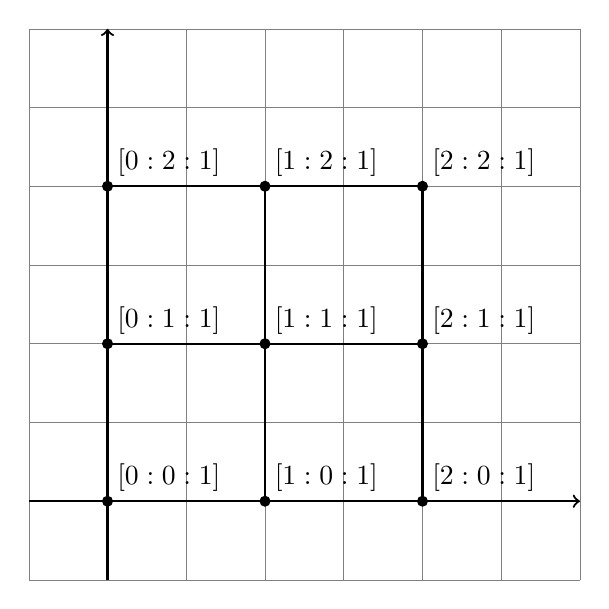
\begin{tikzpicture}
    % Define spacing factor
    \def\spacing{2} % Change this value to adjust spacing

    % Draw grid
    \draw[very thin, gray] (-0.5*\spacing,-0.5*\spacing) grid (3*\spacing,3*\spacing);
    
    % Draw axes
    \draw[thick,->] (-0.5*\spacing,0) -- (3*\spacing,0);
    \draw[thick,->] (0,-0.5*\spacing) -- (0,3*\spacing);

    % Place and label points
    \foreach \x in {0,1,2}
        \foreach \y in {0,1,2} {
            \fill (\x*\spacing,\y*\spacing) circle (2pt);
            \node[above right] at (\x*\spacing,\y*\spacing) {$[\x:\y:1]$};
        }

    % Additional grid lines for structure
    \draw[thick] (0,0) -- (2*\spacing,0);
    \draw[thick] (0,\spacing) -- (2*\spacing,\spacing);
    \draw[thick] (0,2*\spacing) -- (2*\spacing,2*\spacing);
    \draw[thick] (0,0) -- (0,2*\spacing);
    \draw[thick] (\spacing,0) -- (\spacing,2*\spacing);
    \draw[thick] (2*\spacing,0) -- (2*\spacing,2*\spacing);

\end{tikzpicture}



            \end{center}

             We see that any of the points lie on either $x,x-z$ or $x-2z$ and on either $y,y-z$ or $y-2z$. It follows that $f:= x(x-z)(x-2z)$ and $g:=y(y-z)(y-2z)$ are two distinct cubics passing through each of the $9$ points. It follows that $L(f,g)\subset V(3;P_1,\dots,P_9)$, hence $\#V(3;P_1,\dots,P_9)\geq \# L(f,g)=\infty.$
        \end{enumerate}
    \end{example}
    
\subsubsection{Bézout's Theorem}
    \begin{theorem}\label{BezoutTheorem}(Bezout's Theorem)\\
    Let $F$ and $G$ be projective plane curves with no common components. Then 
        $$
            \sum_P I(P, F\cap G) = (\deg \ F)(\deg \ G)
        $$
    \end{theorem}
    \begin{proof}
        By Proposition~\ref{ProjectiveCurvesWithNoCommonComponentsHaveFinitelyManyIntersections} $F$ and $G$ have only finitely many points of intersection. WLOG non of these lie on $L_\infty$. Then 
        $$\sum_P I(P,F\cap G) = \sum_P I(P,F_\ast\cap G_\ast) = \dim\ K[x,y]/\langle F_\ast,G_\ast\rangle.$$
        We define 
        $$
        \begin{matrix}
            \Gamma_\ast := K[x,y]/\langle F_\ast,G_\ast\rangle, && \Gamma:= K[x,y,z]/\langle F,G\rangle, && R = K[x,y,z].
        \end{matrix}
        $$
        We let $\Gamma_d$ denote the space of forms of degree $d$, and $R_d := V(d,3)$ for $d\geq 1$. Set $n:= \deg \ F$ and $m:= \deg \ G.$ It is sufficient to prove that $\dim\ \Gamma_\ast = \dim\ \Gamma_d$ and that $\dim\ \Gamma_d = mn$ for some (large enough) $d$.\\ 
        \textbf{Claim 1:} $\dim\ \Gamma_d = mn$ for every $d\geq m+n$. Consider the 
        sequence 
        $$\begin{tikzcd}
            0 \arrow[r] & R \arrow[r,"\tau"] & R\times R \arrow[r,"\sigma"] & R \arrow[r,"\pi"] & \Gamma \arrow[r] & 0
        \end{tikzcd}$$
        where $\tau: C\mapsto (GC,-FC)$, $\sigma: (A,B)\mapsto AF+BG$ and $\pi$ is the canonical surjection. It is clear that $\sigma \tau=0=\pi\sigma$ hence the sequence is exact. Note that $\tau$ restricts to a linear map from $R_{d-m-n}$ to $R_{d-m}\times R_{d-n}$, that $\sigma$ restricts to a linear map from $R_{d-m}\times R_{d-n}$ to $R_d$ and that $\pi$ restricts to linear map from $R_d$ to $\Gamma_d$. We thus get by exactness (due to Lemma~\ref{DimensionsOfExactSequence}) that 
        \begin{align*}
            &\dim\ \Gamma_d = \dim\ R_d-\dim\ R_{d-m}\times R_{d-n}+\dim\ R_{d-m-n}\\
            &=\frac{(d+1)(d+2)+(-d+m-1)(d-m+2) +(-d+n-1)(d-n+1)+(d-m-n+1)(d-m-n+2)}{2}\\
            &= mn.
        \end{align*}
        Let $\overline{\bullet}$ denote $\bullet + \langle F,G\rangle$.\\
        \textbf{Claim:} The map $\alpha : \Gamma\rightarrow \Gamma, \overline{H} \mapsto \overline{zH}$ is injective. Suppose $zH=AF+BG$. Note that since $z\cap F = \emptyset,z\cap G = \emptyset$, one sees that $F_0:=F(x,y,0)$, $G_0:=G(x,y,0)$ are non-zero forms in $K[x,y]$ that are coprime.\\
        Indeed, suppose $J,I\in K[x_1,\dots,x_{n+1}]$ such that $J(x_1,\dots,x_n,0)\neq 0 \neq I(x_1,\dots,x_n,0)$ have a non-trivial common factor $D$, then $\emptyset\neq H\subset J(x_1,\dots,x_n,0),H(x_1,\dots,x_n,0)$, meaning $x_{n+1}\subset J(x_1,\dots,x_{n+1}),H(x_1,\dots,x_{n+1})$.\\
        Set $A_0:=A(x,y,0)$ and $B_0:= B(x,y,0)$. Then 
        $$A_0F_0 = -B_0G_0.$$
        Hence for some $C\in K[x,y]$, $A_0 = -G_0C$ and $B_0 = F_0C$. Set $A_1 := A+CG$ and $B_1 := B-CF$. Note that 
        $$A_1(x,y,0)=0, \quad B_1(x,y,0) = 0,$$
        hence $A_1= zA'$ and $B_1 = zB'$ for some $A',B'\in K[x,y,z]$, hence 
        $$zH= AF+BG+CFG-CFG = A_1F+B_1F = z(A'F+B'G)\implies H=A'F+B'G\in \langle F,G\rangle$$
        proving that $\ker\ \alpha = 0$.\\
        \textbf{Combining results:} Let $d\geq m+n$ be given. Pick a basis $\{\overline{A_1},\dots,\overline{A_{nm}}\}\subset \Gamma_d$ for suitable $A_i\in R_d$. Consider the restriction of $\alpha$ to $\Gamma_d \rightarrow \Gamma_{d+1}, \overline{H}\mapsto \overline{zH}$, since $\ker\ \left.\alpha\right|_{\Gamma_d} =0$. It follows by rank-nullity that the restriction of $\alpha$ is an isomorphism. Therefor $\{\overline{zA_i}:1\leq i\leq mn\}$ constitutes a basis of $\Gamma_{d+1}$, and by induction $\{\overline{z^rA_i}: 1\leq i\leq mn\}$ form a basis for $\Gamma_{d+r}$ for every $r\geq 0$. We claim that setting $a_i := (A_i)_\ast + \langle F_\ast,G_\ast\rangle,$ $\{a_1,\dots,a_{mn}\}\subset \Gamma_\ast$ constitutes a basis. Let $h = H + \langle F_\ast,G_\ast\rangle\in \Gamma_\ast$, then $\overline{z^NH^\ast}\in \Gamma_{d+r}$ for some sufficiently large $N\geq 0$ and $r\geq 0$, hence 
        $$z^NH^\ast = \sum_1^{mn} \lambda z^rA_i + BF+CG$$ for some $\lambda\in K$, $B,C\in K[x,y,z]$. One then sees that  
        $$H = (z^NH^\ast)_\ast = \sum_1^{nm} \lambda_i (A_i)_\ast+ B_\ast F_\ast+C_\ast G_\ast\implies h = \sum_1^{nm} \lambda_ia_i.$$
        Suppose, $\sum_1^{nm} \lambda_i a_i = 0$. Then $\sum_1^{nm} \lambda (A_i)_\ast = BF_\ast+CG_\ast$ for some $B,C\in K[x,y]$. We then for suitably large $r,s,t\geq0$ that
        \begin{align*}
            z^sB^\ast G + z^tC^\ast = z^r(BF_\ast + CG_\ast)^\ast =z^r\left(\sum_1^{mn} \lambda_iA_i\right)^\ast = \sum_1^{mn}\lambda_iz^{r_i}A_i\sum R_{d+r_i},
        \end{align*}
        implying that $0=\sum_1^{mn} \overline{\lambda_iz^{r_i}A_i}\in \sum \Gamma_{d+r_i}.$ Since $\Gamma_{d+l} \cap \Gamma_{d+k} =0$ (this is seen readily), it follows that $\{z^{r_i}A_i\}$ is a basis of $\sum \Gamma_{d+r_i}$, hence in particular $\{z^{r_i}A_i\}$ are algebraically independent, meaning $\lambda_i=0$. It follows that $\dim\ \Gamma_\ast = \dim \ \Gamma_d = mn.$
    \end{proof}
    \begin{corollary}\label{SumOfMultiplicityBound}
        Let $F$ and $G$ be curves with no common components. Then 
        $$\sum_P m_P(F)m_P(G)\leq (\deg \ F)(\deg \ G).$$
    \end{corollary}
    \begin{proof}
        This follows from property 5 of intersection numbers in conjunction with Bezout's theorem. 
    \end{proof}
    \begin{corollary}
        If $F$ and $G$ (still have no common components) meets in $(\deg\ F)(\deg \ G)$ distinct points, then these points are simple. 
    \end{corollary}
    \begin{proof}
        Under this extra assumption, $m_P(F)m_P(G)\geq 1$ for each point of intersection, meaning $\sum_P m_P(F)m_P(G)\geq (\deg \ F)(\deg \ G)$, hence $\sum_P m_P(F)m_P(G) = (\deg \ F)(\deg \ G)$. Then $m_P(G)m_P(F)=1$ at each point of intersection, for otherwise we would have a strict inequality. We thus conclude that $m_P(F)=m_P(G)=1$ at every point of intersection. 
    \end{proof}
    \begin{corollary}
        If $F$ and $G$ have exactly $(\deg \ F)(\deg \ G)$ common points, then they have no common components.
     \end{corollary}
     \begin{proof}
         This just follows from Bezout and the fact that $\sum_P I(P,F\cap G)<\infty$ if and only if $F$ and $G$ intersect properly at every point. 
     \end{proof}
     \begin{proposition}
         Every non-singular projective curve $F$ is irreducible. 
     \end{proposition}
     \begin{proof}
         Suppose $F$ is reducible with two components $G,H$. $G$ and $H$ have at least one point in common, since if they have a component in common, then they intersect at infinitely many points and if they have no components in common, then by Bezout $\sum_P I(P,G\cap H)=(\deg\ G) (\deg \ H)>1$, meaning they have at least one point in common. Let $P\in G\cap H\subset F$. Then $m_P(F)=m_P(GH)=m_P(G)+m_P(H)\geq 2$, hence $F$ is singular.
     \end{proof}
     \begin{remark}
         It is not the case that the above is true in the affine case. Consider for example $f=y(y+1)$. The zeroes of this curve are $(\alpha,0)$ and $(\alpha,-1)$ where $\alpha\in K$. Since $f(x+\alpha,y+0)=f(x,y)=y^2+y$ and $f(x+\alpha,y-1)=y(y-1)=y^2-y$, hence $f$ is non-singular.
     \end{remark}
     \subsubsection{Bounds on the Number of Multiple Points of a Curve}
     \begin{proposition}
         Let $F$ be an irreducible projective plane curve of degree $d$ with $F_x \neq 0$. Then
         $$\sum_P m_P(F)(m_P(F)-1)\leq d(d-1),$$
         hence $F$ has at most $\frac{d(d-1)}{2}$ multiple points.
     \end{proposition}
     \begin{proof}
         Since $F_x \neq 0$, we have that $\deg \ F_x = d-1$, hence the first bound follows from Corollary~\ref{SumOfMultiplicityBound} and Lemma~\ref{MultiplicityOfPartialDerivative},
         $$\sum_P m_P(F)(m_P(F)-1) \leq \sum_P m_P(F)m_P(F_x) \leq d(d-1)$$.
         Note that the number of multiple points is given by $\sum_P (m_P(F)-1)$. It then follows that
         \begin{align*} 
            2\sum_P(m_P(F)-1) &\leq \sum_{Q \text{ multiple}}\sum_P m_Q(F)(m_P(F)-1)\leq \sum_P m_P(F)(m_P(F)-1) \leq d(d-1).
        \end{align*}
        It thus follows that 
        $$\sum_P (m_P(F)-1)\leq \frac{d(d-1)}{2}.$$
        Another way to derive the bound:
        \begin{align*}
            \sum_P (m_P(F)-1) \leq \sum_P \frac{m_P(F)(m_P(F)-1)}{2} \leq \frac{d(d-1)}{2}.
        \end{align*}
     \end{proof}
     In Example~\ref{ClassifyingCertainCurves} we saw that the optimal bound on the number of multiple points for an irreducible conic is $0$ and for an irreducible cubic $1$, indicating that there is a better bound in the general case. 
     \begin{theorem}
         Let $F$ be an irreducible curve of degree $d\geq 1$. Then 
         $$\sum_P (m_P(F)-1) \leq \frac{(d-1)(d-2)}{2}.$$
     \end{theorem}
     \begin{proof}
         Set
         $$r:= \frac{(d-1)(d-1+3)}{2}-\sum_P \frac{m_P(F)(m_P(F)-1)}{2}\geq \frac{d(d-1)}{2}-\sum_P \frac{m_P(F)(m_P(F)-1)}{2}\geq 0.$$
         Pick $Q_1,\dots,Q_r\in F$ simple. Let $P_1,\dots,P_l\in F$ be the multiple points. Then $$V:=V(d-1; Q_1,\dots,Q_r,(m_{P_1}(F)-1)P_1,\dots,(m_{P_l}(F)-1)P_l)$$
         is a linear subvariety of dimension greater then $\frac{(d-1)(d-1+3}{2}-r-\sum_P \frac{m_P(F)(m_P(F)-1)}{2} =0$. It follows that can pick a curve $G\in V$. Note that if $P\neq Q_i$ is simple, then $m_P(G)\geq 0 = m_P(F)-1$. so $m_P(G)\geq m_P(F)-1$ for each $P\in F$ Since $\deg \ G = d-1 < d=\deg \ F$ and $F$ is irreducible, $\gcd(G,F)=1$, implying 
         \begin{align*}
             r + \sum_{P\neq Q_i} m_P(F)(m_P(F)-1)  &\leq \sum_1^r m_{Q_i}(G)m_{Q_i}(F) +\sum_{P\neq Q_i} m_P(G)m_P(F) \\
             &= \sum_P m_P(G)m_P(F) \leq d(d-1).
         \end{align*}
         Here we use Corollary~\ref{SumOfMultiplicityBound} for the last upper bound. Inserting the value of $r$ into the left-hand side, we see that 
         \begin{align*}
            \frac{(d-1)(d+2)}{2}+ \sum_P \frac{m_P(F)(m_P(F)-1)}{2} \leq \frac{2d(d-1)}{2} \implies &\sum_P \frac{m_P(F)(m_P(F)-1)}{2} \leq\\
            &\frac{(d-1)(2d-d-2)}{2} = \frac{(d-1)(d-2)}{2}. 
         \end{align*}
         We therefor immediately get that $\sum_P (m_P(F)-1)\leq \frac{(d-1)(d-2)}{2}$
     \end{proof}
     \begin{remark}
         This bound is sharp in the cases $d=1,2,3$.
     \end{remark}
     \begin{proposition}
         Let $F$ be a projective plane curve of degree $d\geq 1$ with $c$ components, each of which is not multiple. Then
         $$\sum_P \frac{m_P(F)(m_P(F)-1)}{2}\leq \frac{(d-1)(d-2)}{2}+c-1\leq \frac{d(d-1)}{2}.$$
     \end{proposition}
     \begin{proof}
        write $F=F_1F_2$ where $F_1$ is a component and $F_2$ is a product of $c-1$ remaining simple components with $c>1$. Set $d_1:= \deg\ F_1$ and $d_2:= \deg \ F_2$. By induction and Bezout, it follows that
         \begin{align*}
             \sum_P \frac{m_P(F)(m_P(F)-1)}{2} &= \sum_P \frac{m_P(F_1)(m_P(F_1)+m_P(F_2)-1)}{2} + \sum_P \frac{m_P(F_2)(m_P(F_1)+m_P(F_2)-1)}{2}\\
             &= \sum_1^2\sum_P \frac{m_P(F_i)(m_P(F_i)-1)}{2}+ \sum_P m_P(F_1)m_P(F_2)\\
             &\leq \frac{(d_1-1)(d_1-2)+(d_2-1)(d_2-2)+2d_1d_2}{2} +c-1-1\\
             &= \frac{d_1^2+2-d_1-2d_1+d_2^2+2-d_2-2d_2+2d_1d_2}{2}+c-1-1\\
             &=\frac{(d_1+d_2)^2-(d_1+d_2)-2(d_1+d_2)+2}{2}+c-1\\
             &= \frac{(d-1)(d-2)}{2}+c-1.
         \end{align*}
         Note that in the last step we use $d_1+d_2=d$.
     \end{proof}
     \begin{proposition}
         Assume $\Char \ K=0$. Let $F$ be an irreducible curve of degree $d\geq 1$. Let $P\in \Pp^2$ and set $r=m_P(F)$. For all but finitely many lines $L$ through $P$, $L$ intersects $F$ in $d-r$ distinct points.
     \end{proposition}
     \begin{proof}
         WLOG $P=[0,0,1]$. The lines through $P$ are 
         $$L_\lambda := V(x-\lambda y)= \{[\lambda, 1, t] : t\in K\}\cup \{P\} \quad (\lambda\in K)$$
         (cf. Example~\ref{LinesNotPassingThroughPoints} 1.)
         together with $L = V(y)$. It is therefor sufficient to prove the statement for the $L_\lambda$. Write $F=\sum_r^d H_iz^{d-i}$ with $H_i\in K[x,y]$ a form degree $i$ and $H_r\neq 0$. Consider for each $\lambda \in K$ the polynomial 
         $$G_\lambda := F(\lambda,1,T)\in K[T]$$
         whose roots are in one-to-one correspondence with $L_\lambda \cap F$. It is therefor sufficient to prove that $G_\lambda$ has $n-r$ distinct roots for all but finitely many $\lambda \in K$. Suppose $\lambda\in K$ is given such that $H_r(\lambda,1)\neq 0$ (making $G_\lambda$ a $d-r$-degree polynomial) and $F\cap F_z \cap L_\lambda = \{P\}$, or equivalently that the common roots of $G_\lambda$ and $(G_\lambda)_T=F_z(\lambda,1,T)$ is the empty set. Then by the contrapositive of {\Large result} the $d-r$ roots of $G_\lambda$ are all distinct. Clearly $H_r(\lambda,1)\neq 0$ for all but finitely many $\lambda$. Since $H_i(0,0)=0$ for all $i\geq 1$, it follows that $P \in F_z$. Note that since $F$ is irreducible so is $F(x,1,z)$ by Corollary~\ref{LinearFactoringOfForms}, hence $F(x,1,z)$ and $F_z(x,1,z)$ are co-prime. It then follows that $F(x,1,z)\cap F_z(x,1,z)$ is finite. In particular there are only finitely $\lambda\in K$ such that $\emptyset \neq F(\lambda,1,T) \cap F_z(\lambda,1,T) = G_\lambda \cap (G_\lambda)_T$. It follows that $G_\lambda $ has $d-r$ distinct roots for all but finitely many $\lambda$.
     \end{proof}
     \begin{proposition}
         The above proposition extends to curves $F$ with no multiple components.
     \end{proposition}
     \begin{proof}
         Write $F=\prod_1^n F_i$. Set $r_i := m_P(F_i)$ and $d_i:= \deg \ F_i$. There are infinitely many lines passing through $P$ that do not pass through $\bigcap_1^n F_i$. Denote this set $\pazocal{L}$. Then for each $i$, all but finitely many lines in $\pazocal{L}$, intersect $F_i$ in $d_i-r_i$ points. Then $L$ intersect each $F_i$ in $d_i-r_i$ points for all but finitely many $i$. Let such an $L$ be given. Then  
         $$L\cap F = L \cap \bigcup_1^n F_i = \bigsqcup_1^n L\cap F_i,$$
         hence 
         $$\#(L\cap F) = \#\left(\bigsqcup_1^n L\cap F_i\right) = \sum_1^n d_i-r_i= d -\sum_1^n m_P(F_i)=d-m_P(F)=d-r.$$
    \end{proof}
    \begin{example}
        Suppose $\Char \ K = p >0$. Set $F:=x^{p+1}-y^pz$ and $P:= [0,1,0]$. $L_\infty \cap F = \{P\}$. Let $\lambda \in K$. Then $L_\lambda \cap F= \left\{t : \lambda^{p+1} -t^{p}=0\right\}\cup \{P\} =\left\{ \left[\lambda , 1, \lambda^{\frac{1}{p}}{\lambda}\right]\right\}\cup \{P\}$ {\Large More explicit description?}. Note that 
        $$\begin{cases}
            F_x = x^p\\
            F_y = 0\\
            F_z = y^p
        \end{cases}$$
    \end{example}
\subsubsection{Max Noether's Fundamental Theorem}
    \begin{definition}
        A \textit{zero-cycle} on $\Pp^2$ is an element of the free abelian group generated by $\Pp^2$, i.e. $\Z[\Pp^2]$.
    \end{definition}
    \begin{definition}
        We define the \textit{degree} of a zero-cycle $s=\sum_P n_PP\in \Z[\Pp^2]$ is the quantity
        $$\deg \ s := \sum_P n_P.$$
        For a $t= \sum_P m_P\in \Z[\Pp^2]$, we write $s\geq t$ if $n_P\geq m_P$ for each $P\in \Pp^2$.
    \end{definition}
    \begin{definition}
        Let $F$ and $G$ be curves with no common components. We define the \textit{intersection cycle of $F$ and $G$} to be 
        $$F\ic G:= \sum_P I(P,F\cap G)P\in\Z[\Pp^2]$$
    \end{definition}
    \begin{remark}
        By Bezout $\deg \ F\ic G = (\deg\ F)(\deg \ G)$
    \end{remark}
    The following properties of intersection cycles are trivial consequences of properties of intersection numbers:
    \begin{lemma}
        Let $F,G,H$ be curves and $A$ a form of degree $\deg \ G - \deg \ F$. Then 
        \begin{enumerate}
            \item $F\ic G = G\ic F.$
            \item $F\ic GH = F\ic G + F\ic H.$
            \item $F\ic G + AF = F \ic G.$
        \end{enumerate}
    \end{lemma}
    \begin{definition}
        Consider projective plane curves $F,G,H$ where $F$ and $G$ have not common components. Let $P\in\Pp^2$. We say that \textit{Noether's condition (with respect to $F,G$ and $H$) is satisfied at $P$} if $H_\ast \in \langle F_\ast,G_\ast\rangle \subset \pazocal{O}_P(\Pp^2).$
    \end{definition}
    \begin{theorem}\label{MaxNoethersFundamentalTheorem}(Max Noether's Fundamental Theorem/MNFT)\\
        Let $F,G,H$ be projective plane curves where $F$ and $G$ have no common components. Then there are curves $A$ and $B$ with $\deg \ A = \deg \ H-\deg \ F$ and $\deg \ B = \deg \ H -\deg \ G$ such that 
        $$ H= AF+BG$$
        if and only if Noether's conditions are satisfied at every $P\in F\cap G$.
    \end{theorem}
    \begin{proof}
        "$\implies$": Is trivial\\
        "$\impliedby$": WLOG $F\cap G\cap z=\emptyset$. Since $$K[x,y]/(K[x,y]F_\ast+K[x,y]G_\ast)\simeq \prod_{P=[v,1]\in F\cap G} \pazocal{O}_v/(\pazocal{O}F_\ast+\pazocal{O}_vG_\ast)$$
        and $H_\ast\in \pazocal{O}F_\ast+\pazocal{O}_vG_\ast$ for each $P=[v,1]\in F\cap G$, we get that $H_\ast \in K[x,y]F_\ast+K[x,y]G_\ast$, hence for suitable $a,b\in K[x,y]$, $H_\ast = aF_\ast+bG_\ast$. For a suitably large $N\geq 0$,
        \begin{align*} 
            z^rH=z^N(H_\ast)^\ast &= z^N(aF_\ast+bG_\ast)^\ast = a^\ast z^s(F_\ast)^\ast+b^\ast z^t (G_\ast)^\ast = a^\ast z^{s'}F+b^\ast z^{t'}F,
        \end{align*}
        hence $z^rH=AF+BG$ for suitable forms $A,B\in K[x,y,z]$. By the proof of Bezout, $K[x,y,z]/\langle F,G\rangle \rightarrow K[x,y,z]/\langle F,G\rangle, \Lambda\mapsto z^r\Lambda $ is injective, hence 
        $$H= A'F+B'G$$
        for some $A',B'\in K[x,y,z]$, hence writing $A' = A_{\deg \ H- \deg \ F}'+\dots$ and $B' =B_{\deg \ H- \deg \ G}'+\dots$, as a result of cancellations
        $$H= A_{\deg \ H- \deg \ F}'F+B_{\deg \ H- \deg \ G}'G.$$
    \end{proof}
    \begin{proposition}\label{SufficientConditionsForNoethersCondition}
        Let $F,G,H$ be projective plane curves and $P\in F\cap G$. Noether's condition at $P$ are satisfied if:
        \begin{enumerate}
            \item $F$ and $G$ intersect transversally at $P$ and $P\in H$. 
            \item $P$ is simple on $F$ and $I(P,H\cap F)\geq I(P,G\cap F)$.
            \item $F$ and $G$ have distinct tangents at $P$ and $m_P(H)\geq m_P(F)+m_P(G)-1$.
        \end{enumerate}
    \end{proposition}
    \begin{proof}
        1. Note that 1. implies 2. since then $I(P,H\cap F)\geq 1 = I(P,F\cap G)$, so it is sufficient to prove 2.\\
        2. We get that $\ord^F_P(H)=I(P,H\cap F)\geq I(P,G\cap G)=\ord^F_P(F)$, hence $\pazocal{O}_P(F)\ni \overline{H_\ast} = uL^k$ and $\pazocal{O}_P(F)\ni \overline{G_\ast} = uL^h$ with $h\leq k$, hence $\overline{H_\ast}\in \langle \overline{G_\ast}\rangle \in \pazocal{O}_P(F)$. Then using $\pazocal{O}_P(F)/\langle \overline{G_\ast}\rangle\simeq \pazocal{O}_P(\Pp^2)/\langle F_\ast,G_\ast\rangle$, we find that $H_\ast+\langle F_\ast,G_\ast\rangle =0$.\\
        3. WLOG $P=[0,0,1]$. Note that then $m_P(H_\ast)\geq m_P(F_\ast)+m_P(G_\ast)-1$. This implies that $H_\ast \in \langle x,y\rangle^{m_P(F_\ast)+m_P(G_\ast)-1}$, hence by Lemma~\ref{RadicalOfXYIdeal}, $0=H_\ast+\langle F_\ast,G_\ast\rangle \in \pazocal{O}_{(0,0)}(\A^2)/\langle F_\ast,G_\ast\rangle \simeq \pazocal{O}_P(\Pp^2)/\langle F_\ast,G_\ast\rangle$
    \end{proof}
    \begin{corollary}\label{ExistenceOfSmallerSubCycle}
        Let $F$ and $G$ be projective plane curves with no common components. Then there is a curve $B$ where $B\ic F = H\ic F-G\ic F$ if one of following two conditions are satisfied:
        \begin{enumerate}
            \item $F$ and $G$ intersect in $(\deg \ F)(\deg\ G)$ points and $H$ passes through each of these points.
            \item All points of $F\cap G$ are simple points of $F$ and $H\ic F\geq G\ic F$.
        \end{enumerate}
    \end{corollary}
    \begin{proof}
        If 1. is satisfied, then $F$ and $G$ intersect transversally at every point of intersection, hence by 1. of the prior proposition Noether's condition is satisfied at every point of intersection.\\
        If 2. is satisfied then $I(P,H\cap F)\geq I(P,G\cap F)$, hence 2. of the prior propositions shows that Noether's condition is satisfied at every $P\in F\cap G$.\\
        In either case, this means $H=AF+BG$ for suitable forms $A,B$ by Max Noether's Fundamental Theorem.
    \end{proof}
    \begin{proposition}
        Let $F,G,H$ be plane curves where $\gcd(F,G)=1$, $P\in F\cap G$.
        \begin{enumerate}
            \item When $P$ is simple, then Noether's condition at $P$ is satisfied at $P$ if and only if $I(P,F\cap H)\geq I(P,F\cap G)$.
            \item When $F$ and $G$ meet transversally at $P$, then Noether's condition at $P$ is satisfied at $P$ if and only if $P\in H$. 
        \end{enumerate}
    \end{proposition}
    \begin{proof}
         WLOG $P=[0,0,1]$.
        1"$\implies$": Write $H_\ast = \frac{\alpha}{\beta}F_\ast+\frac{\lambda}{\mu}G_\ast$  for some $\frac{\alpha}{\beta},\frac{\lambda}{\mu}\in\pazocal{O}_{0,0}(\A^2)$. Then 
        $$\zeta H_\ast = \alpha F_\ast + \lambda G_\ast, \quad (\zeta := \beta\mu).$$
            Then 
        \begin{align*}
            I(P,H\cap G)&= I((0,0), H_\ast \cap G_\ast) = I((0,0), \zeta H_\ast\cap G_\ast) = I((0,0), \alpha F_\ast\cap G_\ast)\\
            &= I((0,0), \alpha \cap G_\ast) + I((0,0), F_\ast \cap G_\ast) \geq I((0,0), F_\ast\cap G_\ast) = I(P,F\cap G)
        \end{align*}
        "$\impliedby$": Follows from Proposition~\ref{SufficientConditionsForNoethersCondition}.\\
        2.Follows from 1. 
    \end{proof}
    \begin{remark}
        The above shows that in Proposition~\ref{SufficientConditionsForNoethersCondition} in case 1. resp. case 2. if we presuppose the condition on $F$ and $G$, then the condition on $H$ is equivalent to Noether's condition being satisfied for $F,G$ and $P$. The next example shows that the same augmentation can not be made in case 3.
    \end{remark}
    \begin{example}
        Consider $F=x^2+x+y$, $G=x^2$ and $H=x+y$ and $P=[0,0,1]$. Note that $F$ and $G$ have distinct tangents, namely $x+y$ resp. $x$. One sees that $H_\ast = H=F-G=F_\ast-G_\ast$, so Noether's condition is satisfied at $P$ wrt. $F$ and $G$. Note that $1=m_P(H)<2=m_P(F)+m_P(G)-1$. So the condition on $H$ in case 3. in Proposition~\ref{SufficientConditionsForNoethersCondition} is not equivalent to Noether's condition on $P$ for curves $F,G, H$ with $\gcd(F,G)=1$, $P\in F\cap G$ and $F$ and $G$ having distinct tangents.
    \end{example}
    \begin{proposition}
        Let $F$ be an irreducible projective plane curve. Suppose $z\in K(F)$ is given such that $z\in \pazocal{O}_P(F)$ for every $P\in F$. Then $z\in K$.
    \end{proposition}
    \begin{proof}
        write $z=\frac{H+\langle F\rangle}{G+\langle F\rangle} $, for some equidegree forms $H,G\in K[\mathbf{x}]$, where $G(P)\neq 0$ for every $P\in F$. Then $F\cap G=\emptyset$ hence Noether's condition is vacuously satisfied for every $P\in F\cap G$. Then by MNFT there are forms $A,B\in K[\mathbf{x}]$ such that $\deg \ AF = \deg \ H$, $\deg \ BG= \deg \ H = \deg \ G $. Then $B\in K$ and 
        $$z = \frac{H+I(F)}{G+ I(F)} = \frac{AF+BG+I(F)}{G+I(F)}= \frac{BG+ I(F)}{G+ I(F)}=B+I(F)\in K.$$
    \end{proof}
\subsubsection{Applications of Noether's Theorem}
    \begin{proposition}
        Let $C,C'$ be cubics such that $C\ic C' = \sum_1^9 P_i$. Let $Q$ be a conic such that $Q\ic C = \sum_1^6 P_i$. Assume $P_1,\dots,P_6$ are simple on $C$. Then $P_7,P_8$ and $P_9$ lie on a line.
    \end{proposition}
    \begin{proof}
        Since $P_1,\dots,P_6$ are distinct, $I(P_i,C'\cap C)\geq 1 = I(P_i,Q\cap C)$ for $i=1,\dots,6$. For $i=7,8,9$ (7 8 9?! I guess that's why 6 is afraid of 7), $I(P_i,C'\cap C) \geq 1 \geq I(P_i,Q\cap C)$, since $I(P_i,Q\cap C)=1$ if $P_i\in Q\cap C$ and $0$ otherwise. It follows that $C'\ic C\geq Q\ic C$. By Corollary~\ref{ExistenceOfSmallerSubCycle} there is an $L$ such that $L\ic C = C'\ic C-Q\ic C=P_7+P_8+P_9$. Since $\deg \ C = 3$ and $(\deg\ L)(\deg\ C)= \deg \ L\ic C = 3$, we get that $\deg \ L = 1$, hence $L$ is a line passing through $P_7,P_8,P_9$.
    \end{proof}
    \begin{definition}
        Given $2n$ points in the projective plane $P_1,\dots, P_{2n}$, we form a $2n$-gon by connecting these points via $2n$ lines $L_i:= L(P_i,P_{i+1})$ for $i\in\{1,\dots,2n-1\}$ and $L_{2n}:= L(P_{2n},P_1)$. For the first $n$ lines, we define the \textit{opposite side of $L_i$}, denoted $\mathrm{op}(L_i)$ to be $L_{i+n}$. For the remaining lines, the opposite to $L_i$ is $L_{i-n}$.
    \end{definition}
    \begin{remark}
        Thus we get bijection of any collection of $n$ line segments, $LS$ satisfying that the opposite segment of any $L\in LS$ is not $LS$, to the opposite line segments to those in $LS$, via $\mathrm{op}$. 
    \end{remark}
    \begin{corollary}(Pascal's Theorem)
        Let $Q$ be an irreducible conic (an ellipse, parabola or hyperbola). Pick $6$ distinct points on $Q$, in some ordering $P_1,\dots,P_6$ and form the hexagon containing these points. Then the points $P_i:=L_i\cap\mathrm{op}(L_i)$, $i:=1,2,3$ lie on a line. More generally given a set $LS:= \{L_{i_1},L_{i_2},L_{i_3}\}$, satisfying the conditions of the prior remark, the points $Q_j:= L_{i_j}\cap \mathrm{op}(L_{i_j})$ lie on a line.   
    \end{corollary}
    \begin{proof}
        Indeed, consider the cubics $C:=L_{i_1}L_{i_2}L_{i_3}$ and $C':=\mathrm{op}(L_{i_1})\mathrm{op}(L_{i_2})\mathrm{op}(L_{i_3})$ and apply the prior proposition. 
    \end{proof}
    \begin{corollary}(Pappus' Theorem)
        Let $L_1,L_2$ be two lines, $P_1,P_2,P_3\in L_1$ and $Q_1,Q_2,Q_3\in L_2$ such that $P_i,Q_j\notin L_1\cap L_2$. Set $L_{ij}:= L(P_i,Q_j)$. For each $i,j,k$ with $\{i,j,k\} = \{1,2,3\}$, set $R_k:=L_{ij}\ic L_{ji}$. Then $R_1, R_2,R_3$ lie on a line. 
    \end{corollary}
    \begin{proof}
        Indeed, Consider $Q:= L_1L_2$, $C:=L_{12}L_{13}L_{23}$ and $C':=L_{21}L_{31}L_{32}$. By construction non of the $L_{ij}$'s are components of $Q$. We see that $C\ic C' = \sum_1^3 P_i+Q_i+R_i$ and $Q\ic C = \sum_1^3 P_i+Q_i$ and also note that we chose $P_i,Q_i$ such that they are simple. We are thus in position where we can apply the proposition to see that $R_1,R_2,R_3$ are on a line. 
    \end{proof}
    \begin{proposition}
        Let $C,C',C''$ be cubics with $C$ irreducible, and $Q\in C$. Suppose $C'\ic C=\sum_1^9 P_i$, where the $P_i$ are simple but not necessarily distinct points on $C$ and that $C''\ic C = Q+\sum_1^8 P_i$, then $Q=P_9$. 
    \end{proposition}
    \begin{proof}
         Take any line $L$ passing through $P_9$. Note that $L\ic C= P_9+R+S$ for some $R,S\in C$. Then $LC''\ic C=C'\ic C+Q+R+S$. By Noether's Theorem there is a line $L'$ passing through $Q,R,S$. But then $L=L'$, hence $P_9+R+S = L\ic C=L' \ic C=  Q+R+S$, meaning $P_9=Q$.  
    \end{proof}
    \begin{definition}
        Let $C$ be a non-singular cubic. Take any two points $P,Q$ on $C$. Take the unique line $L$ such that $L\ic C = P+Q+R_{P,Q}$ for some unique $R_{P,Q}\in C$. When $P\neq Q$, $L=L(P,Q)$ and when $P=Q$, $L$ is the tangent at $P$. Define a binary operation on $C$
        \begin{gather*}
            \squareplus: C\times C\rightarrow C\\
            (P,Q)\mapsto R_{P,Q}
        \end{gather*}
    \end{definition}
    \begin{remark}
        With this operation $C$ becomes a commutative magma I.e. $\squareplus$ is a commutative operation.
    \end{remark}
    \begin{definition}
        Let $C$ be a non-singular cubic. Choose any point $O$ on $C$. Define a binary operation 
        \begin{gather*}
            \oplus_{O} := \oplus : C\times C \rightarrow C\\
            (P,Q)\mapsto O \squareplus ( P\squareplus Q)
        \end{gather*}
    \end{definition}
    \begin{proposition}
        Let $C$ be a non-singular cubic. With $\oplus$, $C$ becomes an additive group with $O$ being the identity. 
    \end{proposition}
    \begin{proof}
        We first show that the operation is associative. Let $P,Q,R\in C$. We pick unique lines $L_1,L_2,L_3,M_1,M_2,M_3$ such that 
        \begin{gather*}
            L_1 \ic C = P + Q + P\squareplus Q\\
            L_2 \ic C  = P\oplus Q + R + (P\oplus Q)\squareplus R\\
            L_3 \ic C = O + Q \squareplus R + \underbrace{ O \squareplus (Q \squareplus S)}_{Q \oplus R}\\
            M_1 \ic C = O + P \squareplus Q + \underbrace{ O \squareplus ( P \squareplus Q ) }_{P\oplus Q}\\
            M_2 \ic C = Q + R + Q \squareplus R\\
            M_3 \ic C = P + Q \oplus R + P \squareplus ( Q\oplus R)
        \end{gather*}
        Set $C' := L_1L_2L_3$ and $C'' := M_1M_2M_3$. Then 
        \begin{gather*}
            C'\ic C = O+P+Q+R+P \squareplus Q + Q \squareplus R + P \oplus Q + Q \oplus S + (P\oplus Q)\squareplus R,\\
            C'' \ic C = O+P+Q+R+P \squareplus Q + Q \squareplus R + P \oplus Q + Q \oplus S + P\squareplus(Q\oplus R).
        \end{gather*}
        Applying the prior proposition, it follows that $(P \oplus Q)\squareplus R = P \squareplus (Q\oplus R)$. Then $O+(P \oplus Q)\squareplus R (P\oplus Q)\oplus R = O+ P \squareplus (Q\oplus R) + P\oplus (Q\oplus R)$, hence $(P\oplus Q)\oplus R = P\oplus (Q\oplus R)$. Moreover, the line through $O$ and $O\oplus P$ is the line through $O$ and $P$, hence $O\oplus P = P$. Define $-P := P\squareplus (O \squareplus O)$. Then the third intersection of $C$ with the line through $P$ and $-P$ is $O\squareplus O$. Moreover the third point of intersection of $C$ with the line through $O$ and $O\squareplus O$ is $O$, hence $P\oplus -P = O\squareplus (P \squareplus -P)= O \squareplus (O\squareplus O)= O$. Commutativity, follows from commutativity of $\squareplus$.
    \end{proof}
    \begin{definition}
        Let $C$ be a cubic with no multiple components. Define 
        $$C^o := \{ P\in C : P \text{ simple} \}.$$
    \end{definition}
    \begin{remark}
        When $C$ is irreducible, we may define $\squareplus$ as in the non-singular case, since $L(P,Q)$ is not a component of $C$ in this case there is a unique point $R_{P,Q}$ such that $L(P,Q)\ic C = P+Q+R_{P,Q}$. We see that $I(R_{P,Q}, L(P,Q)\cap C)=1$, hence $R_{P,Q}$ is simple, meaning $\squareplus$ is indeed well-defined. Pick a point $O\in C^o$. Upon for $P,Q\in C^o$ defining, $P\oplus Q := O \squareplus (P \squareplus Q)$, the same computations as in the nonsingular case shows that $(C^o,\oplus)$ is an additive group.\\
        If $C$ has a non-trivial component {\Large Then I don't know}.
    \end{remark}
    \begin{proposition}
        Consider an irreducible cubic $C$. Let $O,O'\in C^\circ$ be given. Set $Q:= O\squareplus O'$. Then 
        \begin{gather*}
            \alpha : (C^\circ, \oplus_O) \rightarrow (C^\circ, \oplus_{O'})\\
            P \mapsto Q \squareplus P
        \end{gather*}
        defines a group isomorphism. 
    \end{proposition}
    \begin{proof}
        
    \end{proof}
    \begin{proposition}
        Let $P_1,P_2,P_3$ be distinct points on an irreducible conic $Q$. Let $L_1,L_3,L_5$ be the tangents at each of the respective points. Let $L_{2}:=L(P_1,P_2)$, $L_4:= L(P_2,P_3)$ and $L_6:= L(P_3,P_1)$. Then $Q_i := L_i\cap \mathrm{op}(L_i)=L_i\cap L_{i+3}$ for $i=1,2,3$ are collinear
    \end{proposition}
    \begin{proof}
        Set $C=L_{1}L_{3}L_{5}$, $C':= L_2L_4L_6$. For each $i$ note that there are exactly two lines in $C'$ intersecting $P_i$. Since neither of these points are tangents to $Q$, they intersect the tangent to $P_i$ transversally. It follows that $I(P_i,C\cap C')= 2$, hence 
        $$C\ic C' = \sum_1^3 2P_i+Q_i.$$
        Additionally 
        $$Q\ic C' = \sum_1^3 2P_i,$$
        it follows from a Corollary~\ref{ExistenceOfSmallerSubCycle} 2. that there is a line $L$ for which $L\ic C' = \sum_1^3 Q_i$, hence $Q_1,Q_2,Q_3$ are collinear.
    \end{proof}
    \begin{proposition}
        Let $P_1,\dots,P_5$ be distinct points on an irreducible conic $Q$. Let $L_1$ be the tangent at $P_1$ and connect the points with $5$ lines $L_i$ as before. Defining $Q_1,Q_2,Q_3$ as before, we get that these are collinear. 
    \end{proposition}
    \begin{proof}
        Define $C$ and $C'$ as before. Then 
        $$C\ic C' = 2P_1 + \sum_2^5 P_i+ Q_1+Q_2+Q_3$$
        and 
        $$C\ic Q= 2P_1 + \sum_2^5 P_i.$$
        We get a line through $Q_1,Q_2,Q_3$ in the usual way. 
    \end{proof}
    \begin{remark}
        The above result gives a way to construct a tangent to a point on an irreducible conic using only a straightedge: Call the point $P$. Draw $4$ other distinct points also distinct from $P$. Call these points $P_1,\dots,P_4$. Find the intersection of the line $L(P_4,P)$ and $L(P_1,P_2)$. Call that point $Q_1$. Do the same with $L(P_1,P)$ and $L(P_3,P_4)$. Call that point $Q_2$. Find the intersection of $L(P_2,P_3)$ and $L(Q_1,Q_2)$. Call that point $Q_3$. Then $L(P,Q_3)$ is the tangent of the conic at $P$. 
    \end{remark}
    \begin{proposition}
        Consider the hexagon formed by points $P_1,\dots,P_6$. Suppose the intersections of the sides with their opposite side lie on a line.  Then $P_1,\dots, P_6$ lie on a conic.  
    \end{proposition}
    \begin{proof}
        
    \end{proof}
    \begin{proposition}
        Let $C$ be an irreducible cubic and $L$ a line such that $L\ic C = P_1+P_2+P_3$ for $P_1,P_2,P_3$ distinct. Let $L_i$ be the tangent to $C$ at $P_i$. Then $L_i\ic C= 2P_i+Q_i$ for some $Q_i$. Then $Q_1,Q_2,Q_3$ are collinear. 
    \end{proposition}
    \begin{proof}
        
    \end{proof}
    \begin{proposition}
        On a cubic, a line through two flexes on the cubic, passes through a third flex on the cubic.
    \end{proposition}
    \begin{proof}
        
    \end{proof}